\chapter{Dynamic Molecular Docking}

Significant parts of this chapter have been published in \cite{
dmd_samsonov_gehrcke_2014}.

\section{Abstract}
We present Dynamic Molecular Docking (DMD), a novel
targeted molecular dy\-namics-based protocol developed to address ligand and
receptor flexibility as well as the inclusion of explicit solvent in local
molecular docking. A class of ligands for which docking performance especially
benefits from overcoming these challenges are glycosaminoglycans (GAGs). GAGs
are periodic, highly flexible and negatively charged polysaccharides playing an
important role in the extracellular matrix via interaction with proteins such as
growth factors and chemokines. The goal of our work has been to develop a proof
of concept for an MD-based docking approach and to analyze its applicability for
protein-GAG systems. DMD exploits the electrostatics-driven attraction of a
ligand to its receptor, treats both as entirely flexible and considers solvent
explicitly. We show that DMD has high predictive significance for systems
dominated by electrostatic attraction and demonstrate its capability to reliably
identify the receptor residues contributing most to binding.

\section{Rational}
Molecular docking has been extensively applied for drug
discovery in the recent decades \cite{klebe_recent_2000,
cheng_structure-based_2012}. Whereas molecular docking methodologies demonstrate
to be very successful and continue to develop rapidly, they still suffer from a
number of limitations \cite{moreira_proteinprotein_2010,
andrusier_principles_2008,lensink_docking_2010}. What holds true for practically
all docking methods is that the reproduction of an experimentally observed
docking pose is less challenging than proper scoring of this pose by energy
\cite{kim_assessment_2008, plewczynski_can_2011,smith_csar_2011}. In the
majority of docking approaches, only small ligands can be treated as entirely
flexible in order to limit the size of the conformational search space. Although
flexible treatment of the ligand is crucial for obtaining meaningful results,
ligand flexibility often can only be approximated, especially in protein-protein
docking \cite{ritchie_recent_2008}. Another severe approximation applied in most
docking methods is static treatment of the receptor even though protein side
chain flexibility is crucial for ligand binding, and substantial conformational
changes can occur in the receptor structure induced by interaction with a ligand
\cite{gunasekaran_how_2007,gutteridge_conformational_2005}. Finally, most of the
established docking approaches do not explicitly account for solvent molecules,
whereas many studies point out their importance in docking calculations
\cite{van_dijk_solvated_2006,baron_water_2010,roberts_ligandprotein_2008,
thilagavathi_ligand-protein_2010}.

A particularly challenging class of ligands for which docking
performance is especially limited by the above-mentioned issues are
glycosaminoglycans (GAGs), which are periodic negatively charged linear
polysaccharides mainly located in the extracellular matrix. Through interaction
with their protein targets they participate in a number of key processes
involved in cell regeneration and proliferation, angiogenesis, metastasis and
lipid metabolism \cite{hynes_extracellular_2009, macri_growth_2007,
barbero_chembiochem_2013}. Due to the occurrence of numerous sulfate and
carboxyl groups, GAGs have a high charge density, rendering long-range Coulomb
interactions to be crucial for binding to proteins
\cite{mulloy_specificity_2005}. The significance of electrostatic interactions
underlines the importance of taking explicit solvent molecules as binding
mediators into account when GAGs are used as ligands in molecular docking
\cite{samsonov_docking_2011}. Moreover, the orientation and conformation of long
side chains of charged protein residues may be greatly influenced by interaction
with a GAG ligand. In consequence, flexible treatment of the receptor during
GAG-docking is of special relevance. In addition, a similar spatial distribution
of functional groups in GAGs independent of the reducing/non-reducing end
orientation \cite{forster_computational_2006} as well as their high flexibility
\cite{bitomsky_docking_1999} substantially contribute to the challenges in
protein-GAG docking. Overall, the prediction of protein-GAG complexes via
molecular docking comprises a good example of some of the current limitations in
the field of classical molecular docking.

Classical docking approaches are generally optimized for having relatively
modest computational requirements and therefore enable the quick investigation
of single complexes as well as the execution of large-scale studies involving a
large number of different complexes. Taking into account ligand and receptor
flexibility as well as treating solvent explicitly clearly increases the
computational complexity of docking approaches. However, in view of the ever-
increasing computing power, a new generation of docking methods should evolve,
which though being computationally more demanding, aims to deal with the above-
mentioned challenges.

Molecular dynamics (MD) techniques are established for rigorous studies of
intermolecular interactions\cite{karplus_molecular_2005}. Beyond that, MD
methods have already been used in docking approaches for overcoming the
challenges of both ligand and receptor
flexibility\cite{chaudhuri_application_2012, antes_dynadock_2010}. Furthermore,
standard MD methods allow for the inclusion of explicit solvent via well-
established water models. The application of MD techniques is limited by high
computational cost, which previously has hindered their usage in high-throughput
approaches for drug discovery. However, nowadays, advanced computational
resources are available and specialized hardware (such as graphics processing
units, GPUs) can be used to dramatically increase the performance of MD
simulations, making the establishment of MD in the field of docking gradually
feasible.


We propose Dynamic Molecular Docking (DMD), a combination of established MD-
based methods specifically designed for tackling the above-mentioned challenges
in protein-GAG docking. DMD is a targeted MD-based approach where the ligand,
which is initially placed at a distance from the receptor so that their
interaction is negligible, is slowly pulled towards a receptor target region by
applying a time-dependent distance restraint. During this process, both receptor
and ligand are treated as entirely flexible in explicit solvent. The time-
dependent distance restraint applied in DMD is usually used in steered molecular
dynamics simulations, which are performed for studying the energetics of
processes that generally happen on timescales too large for being treated by
classical MD simulations \cite{xiong_free_2006}, such as protein folding, ligand
unbinding and large-scale conformational alteration. In DMD, once the ligand
reaches the receptor, the distance restraint is switched off and a long free MD
simulation is carried out, allowing for the mutual adjustment of receptor
residues and GAG as well as for extensive GAG-internal degree of freedom
sampling. The obtained trajectory data are then used for extracting a docking
solution (the coordinates) and for its characterization (binding energy estimate
and other quantities). Binding pose search as well as binding pose scoring are
consistent in terms of using the same potential as given by the MD force field
and the parameterization of the molecular system.

In this validation study, we applied DMD to a set of reference systems and
compared its performance to a classical docking approach, AutoDock 3 (AD3),
which has successfully been applied to protein-GAG systems before
{\cite{japan_docking_ad3_clustering, samsonov_docking_2011,
pichert_characterization_2012}}. The results obtained for our test data set
comprised of five protein-GAG complexes, one protein-peptide and one protein-
small molecule complex show that DMD has high predictive significance while
performing best when complex formation is driven by strong electrostatic
interaction. Detailed analysis of the electrostatic potential of the
corresponding binding sites, of the spatial distribution of docking solutions,
and per-residue binding free energy decomposition support the promising
potential of the DMD approach when used for docking in highly flexible and
electrostatics-driven systems.

\begin{figure}
\centering
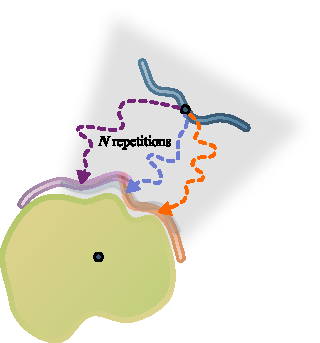
\includegraphics[height=7cm]{gfx/dmd/scheme_n_repetitions_for_thesis_002.pdf}
\caption[]{Schematic representation of the DMD pulling process. Starting from a
distal position, the ligand (blue) is pulled towards its receptor (green).
During this process, the ligand moves along a random path. The pulling process
is repeated $N$ times in independent simulations. Most of the resulting ligand
trajectories lie within a certain \enquote{entry lane}, as depicted here in grey
shade. Each pulling process yields an individual final ligand state (purple,
blue, orange) near the receptor surface.}
\label{fig:dmd:n_repetitions}
\end{figure}


\section{General method description}
\subsection{Data production}

A DMD study for a given receptor-ligand complex implies performing $N$ (e.g.
100) independent DMD runs. The number of independent repetitions $N$ must be
large enough for obtaining convergence regarding certain ensemble properties.
Each DMD run starts with a randomly oriented ligand molecule placed at a
distance from the receptor (ligand re-oriented model, LROM). The first step of a
DMD run is a targeted molecular dynamics (tMD) simulation in which the ligand is
pulled towards a pre-defined target region on the receptor via a time-dependent
decrease of the distance $d(t)$ between one central atom in the ligand and one
core atom in the protein receptor. Among DMD run repetitions, most of the ligand
trajectories lie within a certain \enquote{entry lane} which is focused on a
point near the receptor surface, the focus point $\bm{F}$, and therefore
defining the target region (\cref{fig:dmd:n_repetitions}). All final tMD states
have the central ligand atom positioned on the surface of a sphere defined by
the protein core atom (the center of the sphere) and the final distance $D$ of
the tMD pulling process (the radius of the sphere). Based on the final state of
each tMD simulation, the second step of a DMD run relaxes the system via a free
MD simulation. Geometrical definitions, system preparation, and details about
tMD and free MD parameterization as well as subsequent trajectory data analysis
methods are provided in the following sections.

\begin{figure}
\centering
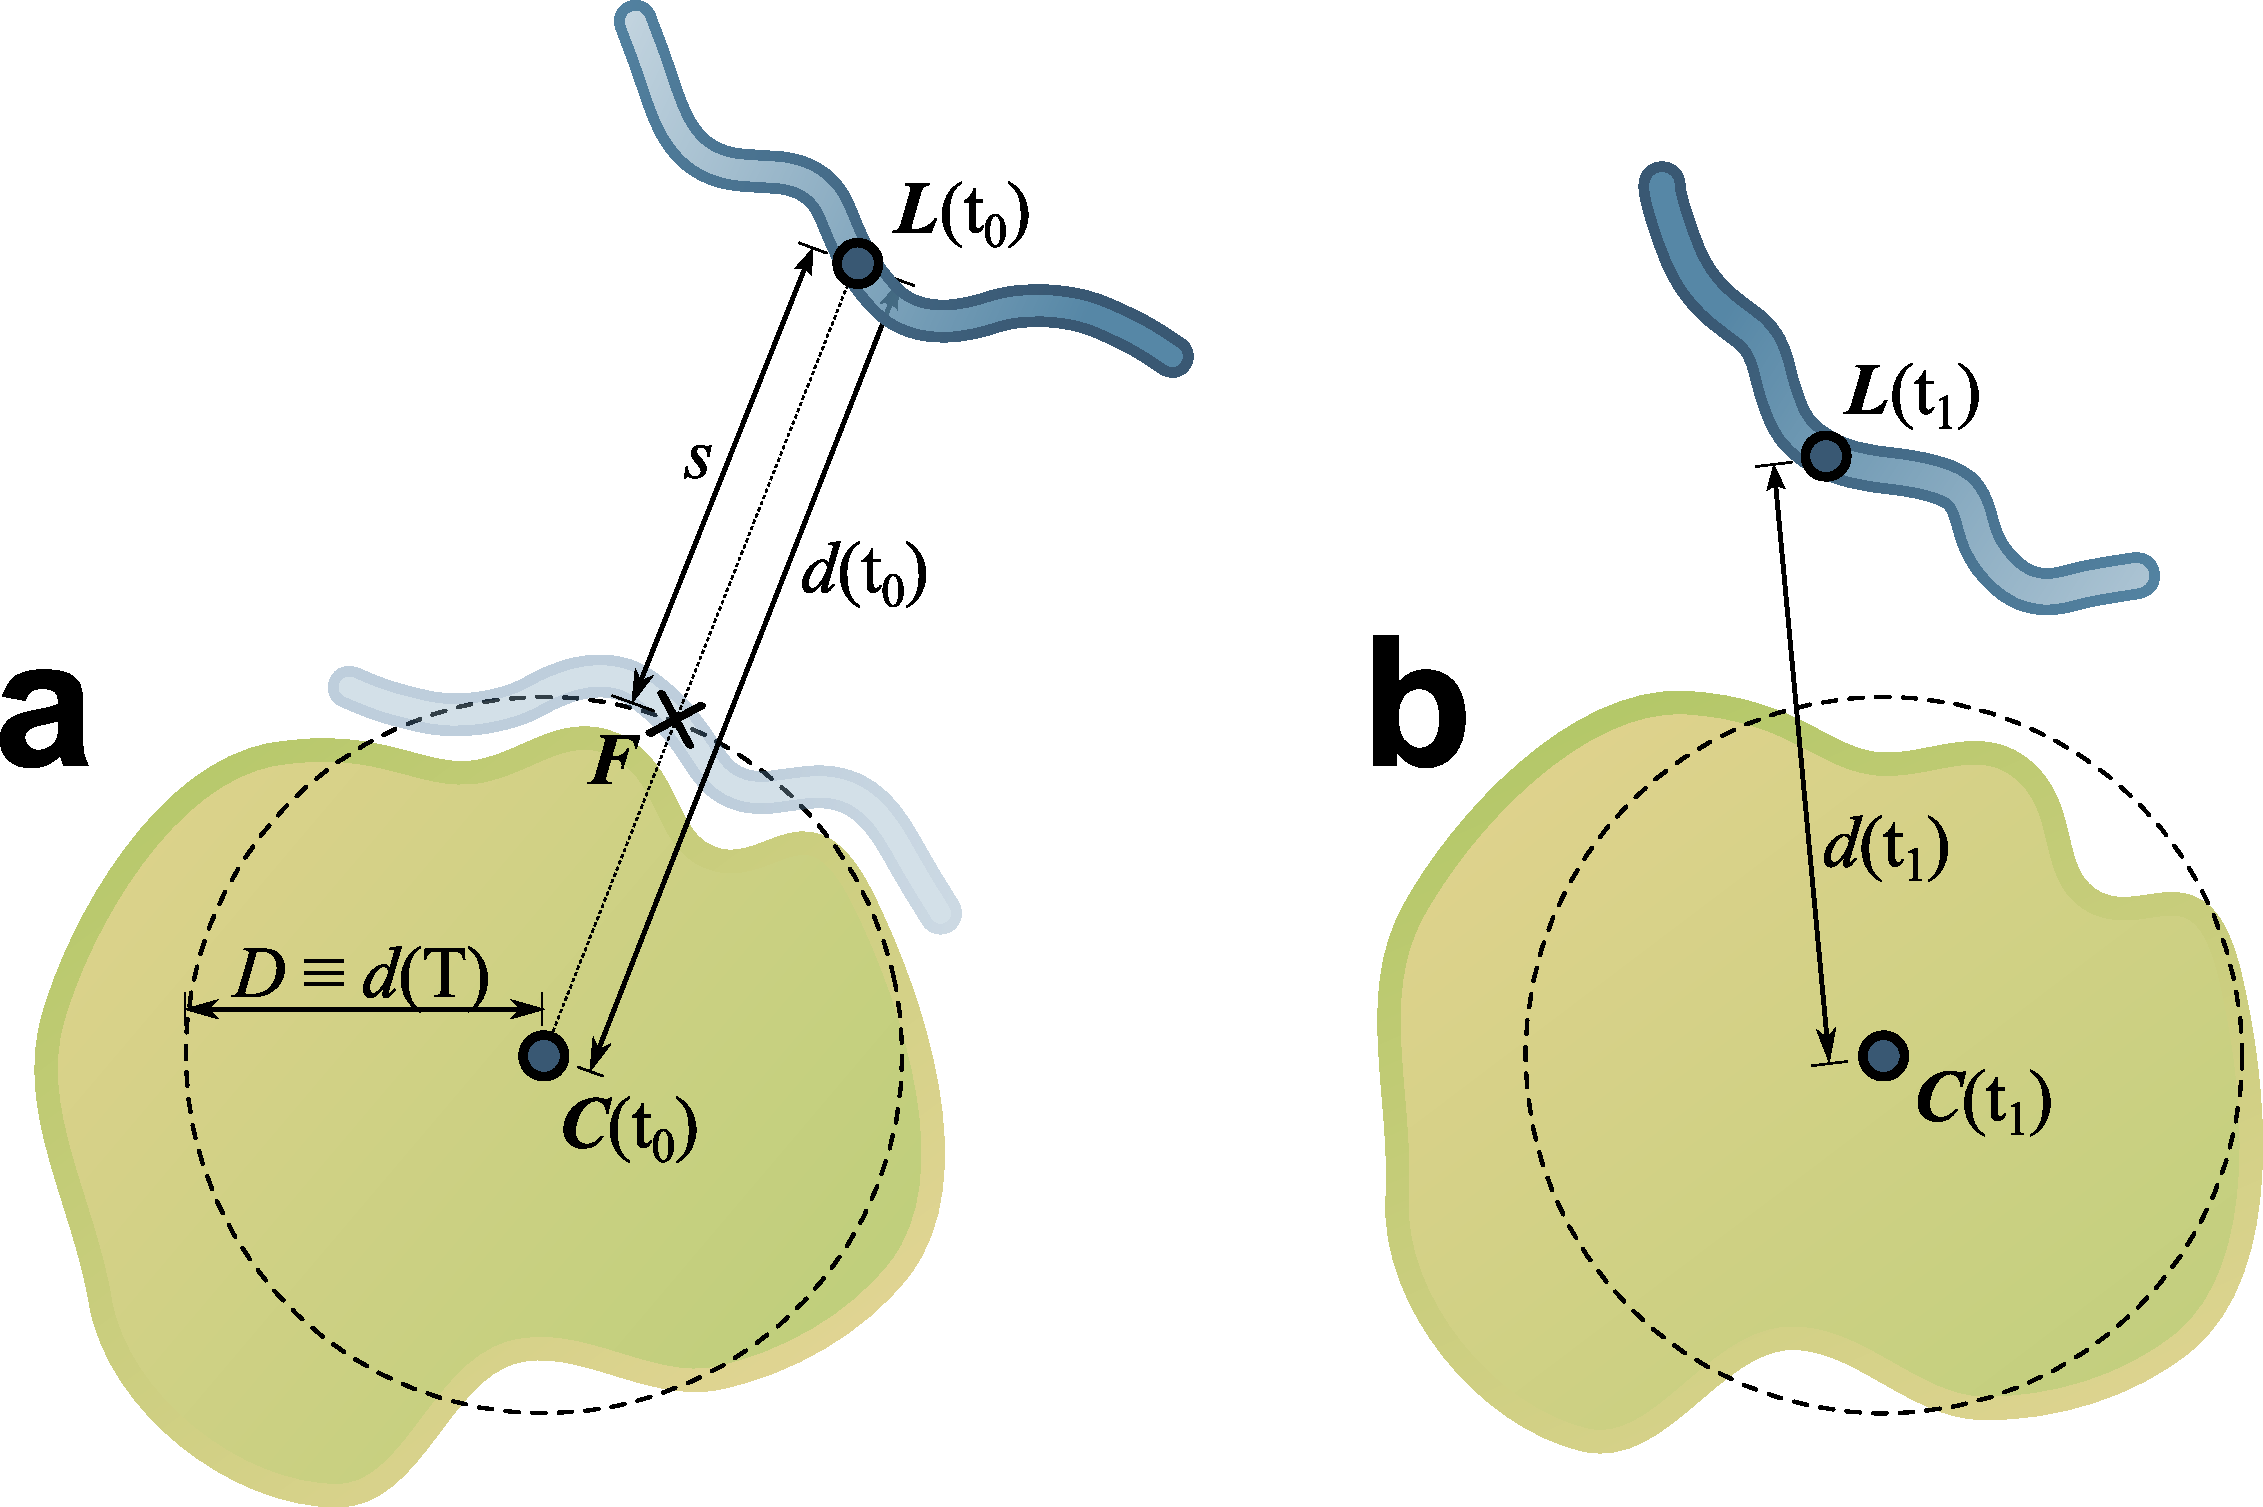
\includegraphics[height=7cm]{gfx/dmd/scheme_geometry_two_panels_002.pdf}
\caption[]{
\textbf{a}: System configuration at time $t_0$ right before the pulling process,
referred to as the ligand-reoriented model (LROM, with the displaced ligand in
dark blue). The central atom of the experimentally determined ligand position
(light blue) has been placed to a distal position $\bm{L}(t_0)$ along the axis
given by a receptor core atom at point $\bm{C}(t_0)$ and the focus point
$\bm{F}$. $s$ is the displacement length. The ligand has been randomly rotated
around its central atom. The distance between $\bm{C}(t_0)$ and $\bm{F}$ defines
the final distance $D$ for the ligand pulling process. The initial distance
$d(t_0)$ between $\bm{C}$ and $\bm{L}$ is $D+s$.
\textbf{b}: arbitrary state within the pulling process, during which the
distance $d(t)$ between central ligand atom at point $\bm{L}(t)$ and protein
core atom at point $\bm{C}(t)$ is decreased over time $t$. Right after the
pulling process, all final ligand states have their central atom placed on the
sphere that is indicated here with a dashed line.
}
\label{fig:dmd:geometry_scheme}
\end{figure}

\subsubsection{Preparation of ligand-reoriented models (LROMs)}
An LROM contains
the receptor as well as the ligand placed in a distal, re-oriented position. Per
TDS complex, ten LROMs have been created, differing only in ligand orientation
around its central atom. For a given complex, LROM creation requires the
selection of a \textit{central ligand atom}, definition of a \textit{focus
point} $\bm{F}$ near the surface of the receptor within the anticipated binding
region, definition of a \textit{ligand displacement length} $s$ and selection of
a \textit{core atom} at point $\bm{C}$ within the receptor. The distance between
focus point and core atom defines the final distance $D$ of the tMD pulling
process, i.e.\  $d(T) \equiv D \equiv  \lVert \bm{F}-\bm{C} \rVert$. Initially,
at time $t_0$, the ligand is placed distal from the receptor with its central
atom lying on the axis defined by $\bm{F}-\bm{C}$
(\cref{fig:dmd:geometry_scheme}a). The starting coordinate for the central
ligand atom is defined as

\begin{equation}
\bm{L}(t_0) = \bm{F} + s \frac{\bm{F}-\bm{C}}{D}.
\end{equation}

For each TDS complex, multiple LROMs should be prepared as follows. First, the
structure of the biological unit of the protein receptor is to be taken from the
corresponding experimental data source (3D structure from crystallography or
NMR). The coordinates of a central atom in the ligand as found in the
experimentally determined structure are to be used as focus point. The core atom
in the receptor must be selected fulfilling three criteria: \textit{i)} it is a
backbone atom within a helix or beta sheet in the protein core, \textit{ii)} the
line connecting core atom and $\bm{F}$ (defining the orientation of the ``entry
lane'' is roughly perpendicular to the surface comprising the anticipated
binding region, and \textit{iii)} the surface of the sphere around the core atom
with radius $D$ has significant overlap with the molecular receptor surface in
the receptor target region. Distal ligand placement is to be followed by
multiple random ligand rotations uniformly distributed in 3D space with
$\bm{L}(t_0)$ being the rotation center. Each rotational ligand corresponds to
one LROM.

\subsection{Data analysis}

            MMPB(GB)SA
            Movement
            H-bonding

\lipsum[1-2]



\section{Implementation for this project}

\subsection{Molecular dynamics protocol}

The DMD-related molecular dynamics simulations performed in the context of this
PhD project were set up, performed, and analyzed using Amber 12 and AmberTools
12 \cite{case_amber_11}. The FF99SB force field was used for parameterization of
the peptidic parts in the investigated complexes. GAG force field parameters
were created based on GLYCAM 06 version g \cite{kirschner_glycam06:_2008} and
sulfate partial charges obtained by RESP fitting calculations at the level of
6-31(d)G for methylsulfate. All systems were solvated in a box of TIP3P water
with a minimum of $8\,\angstrom$ distance between solute and box boundaries. The
systems were neutralized by adding Na$^{+}$ or Cl$^{-}$ counterions. The MD time
integration step was set to $2\,\mathrm{fs}$, whereas bonds including hydrogen
atoms were length-constrained by the standard SHAKE method. During MD,
non-bonded interactions were switched off for atom pairs further apart than
$8\,\angstrom$. The Particle Mesh Ewald method was used for treating long-range
electrostatic interactions.

Each simulated system went through minimization, heat up, equilibration, and
production steps. During the first stage of minimization, only the solvent was
relaxed. During the second stage, the entire system was minimized without
restraints. System heat up to $300\,\mathrm{K}$ was performed within
$20\,\mathrm{ps}$ in the canonical ensemble (NVT) using the Langevin thermostate
and periodic boundary conditions. Subsequently, $500\,\mathrm{ps}$ of MD in the
isothermal-isobaric ensemble (NPT) with Langevin thermostate and Berendsen
barostat under periodic boundary conditions were carried out for system density
equilibration. The following production stage of duration $T$ was performed in
the NVT ensemble with the Berendsen thermostat and periodic boundary conditions.

%For complexes involving heparin, weak torsional restraints were
%applied in order to keep the pyranose rings of IdoA(2S) in the $^{1}C_4$
%conformation. This conformation has been shown to be one of the two
%predominantly populated ones{\cite{almond_jacs_2010}} and was observed
%experimentally in the structure of the FGF2-HP complex in our test data set (PDB
%ID 1BFB). The applied restraints enable to define and control the specific
%%conformation of each IdoA(2S) ring throughout the entire DMD study, since its
%natural ring conformer population is not properly reproduced by GLYCAM
%06{\cite{gandhi_idoa2s_2010}}.

\subsubsection{Targeted and free molecular dynamics.}
The LROMs were prepared for MD and time-evolved following the general MD
protocol as described above. During the tMD production stage, core atom and
ligand center atom were exposed to an additional time-dependent harmonic
potential

\begin{equation}
U(t) = \frac{1}{2} k \left( d(t)-d(t_0) + vt   \right)^2
\end{equation}

with force constant $k=200\,\mathrm{kcal\,mol^{-1}\,A^{-2}}$, pulling velocity
$ v = s/T$ and

\begin{equation}
d(t) = \lVert \bm{L}(t)-\bm{C}(t) \rVert.
\end{equation}

This potential enforces the distance between the selected ligand center atom and
the protein core atom to linearly decrease with time $t$ in the interval from
$D+s$ to $D$ (\cref{fig:dmd:geometry_scheme}b). For all tMD simulations, we used
a pulling velocity of $s=30\,\angstrom$ per $T=4\,\mathrm{ns}$.

For each DMD study, we prepared ten LROMs. Within such a study, we usually
repreated the tMD pulling process 10 to 30 times for each of the LROMs, using a
different random seed for each MD simulation. In total, this yields 100 to 300
independent tMD simulations per DMD study. Based on the final state of receptor
and ligand of each tMD trajectory, an MD simulation with $T=10\,\mathrm{ns}$
without restraints was performed according to the protocol described above,
hereafter referred to as \textit{free MD}.


\subsection{Energetic evaluation of DMD docking results}

From the last 200 ps of each free MD trajectory, 100 equidistantly distributed
frames were extracted for energy analysis. The MM-PBSA \cite{mmpbsa_py} approach
was applied for calculating the time-averaged Coulomb interaction energy $\Delta
E$ between receptor and ligand as well as an estimate for the free energy of
binding $\Delta G$. MM-GBSA\cite{mmpbsa_py} single residue energy decomposition
(SRED) was applied to estimate the energy contribution of single receptor
residues to the bound state.

In order to identify the receptor residues mostly contributing to the binding
from all 100 DMD runs corresponding to one TDS complex, the SRED data of all
free MD trajectories were filtered and merged: we excluded DMD runs resulting in
weakly bound docking solutions (MM-PBSA $\Delta G >
-1\,\mathrm{kcal\,mol^{-1}}$) and averaged the SRED-energy $\Delta G_R$ for each
receptor residue over the remaining independent DMD runs. We discarded all
receptor residues with an average SRED-energy $\langle\Delta G_R\rangle \ge
0\,\mathrm{kcal\,mol^{-1}}$ and ranked the remaining ones by $\langle\Delta
G_R\rangle$. For each TDS complex, we extracted the 10 top-ranked residues,
referred to as the set of receptor \textit{anchoring residues}. For reference,
we set up an identical MD simulation ($T=10\,\mathrm{ns}$) of each
experimentally determined TDS complex and used SRED to obtain a set of reference
anchoring residues for comparison.

MM-PBSA free energy calculations as well as MM-GBSA single residue energy
decompositions were performed with default parameters using the Python version
of the MM-PBSA application provided with AmberTools 12. We did not consider an
entropic contribution to binding since we aimed to compare very similar systems
where taking into account entropy may increase the overall uncertainty in the
calculated binding energies{\cite{Gandhi01102009, homeyer_gohlke_2012}}.

\subsection{Software architecture}
\lipsum[1-2]


\subsection{Computing resources}

Most of the simulations were performed on a compute cluster comprised of AMD
Opteron 6274 CPUs. On these machines, a DMD study as
described above requires about 100.000 CPU hours per TDS complex.
For testing purposes, some MD simulations were executed on Nvidia Tesla C2070
as well as Nvidia GTX 580 GPUs, taking advantage of Amber's recent optimizations
for such hardware \cite{amber_gpu_2012}.

\lipsum[1-2]


\section{Validation study}
\subsection{Methods}
\subsubsection{Test data set}

Seven protein-ligand complexes with experimentally determined 3D structures were
used as test data set (TDS). Five of them are protein-GAG systems: basic
fibroblast growth factor (FGF2) in complex with a heparin (HP) tetrasaccharide,
PDB ID 1BFB, 1.9 Å resolution; cathepsin K (CathK) in complex with a
chondroitin-4-sulfate hexasaccharide (CS4), PDB ID 3C9E, 1.8 Å; a CathK mutant
(referred to as CathKmut) in complex with a CS4 hexasaccharide, PDB ID 3H7D, 2.2
Å; CD44 in complex with a hyaluronan heptasaccharide (HA), PDB ID 2JCQ, 1.3 Å;
stromal cell-derived factor-1 (SDF-1) in complex with a HP disaccharide, PDB ID
2NWG, 2.1 Å. In our studies we also included two complexes of different nature:
Abl-SH3 domain complexed with a decapeptide (p41), PDB ID 1BBZ, 1.7 Å; trypsin
in complex with the inhibitor benzo[b]thiophene-3-methanamine (referred to as
Ihb.), taken from the DINGO dataset \cite{newman_dingo_2012}.

\subsubsection{Classical molecular docking}

For comparison with DMD, classical docking based on AutoDock
3\cite{morris_automated_1999} (AD3) was applied to all TDS complexes. AD3 has
been shown to produce reasonable results for GAG-protein systems, especially
compared to other docking methods  \cite{japan_docking_ad3_clustering,
samsonov_docking_2011, imberty_perez_protgag_comp_book_2006,
franz_cathepsin_2013}.

With AD3, a semi-flexible ligand is docked to a static receptor without presence
of explicit solvent. In order not to be biased towards a ligand-induced receptor
conformation, prior to docking with AD3, we relaxed all TDS receptor structures
via energy minimization in the Amber 99 force field as implemented in MOE
\cite{chemical_computing_group_inc_moe_2010} using a convergence criterion of
$0.01\,\angstrom$ heavy atom $RMSd$.

For each TDS complex, the potential grid of the receptor was calculated with a
grid step of $0.38\,\angstrom$. Grid size, position and orientation were chosen
so that the spatial sampling volume is comparable to the one in DMD. We set
ligand torsional degrees of freedom for glycosidic linkages as well as sulfate
and carboxyl groups to be flexible during the search. $10^3$ independent docking
runs were performed for each complex. Each docking run was performed by a
genetic algorithm (initial population size: 300, abortion condition: $10^5$
generations) followed by a local search. If not stated otherwise, default
parameters were used. Spatial clustering was performed with the top 100
solutions according to the AD3 score.

\subsubsection{Spatial clustering of docking results}
In order to evaluate the spatial distribution of docking solutions generated by
either docking method, we used the DBSCAN clustering algorithm
\cite{dbscan_ester1996}. Based on the  parameters $\epsilon$ (neighborhood
search radius) and $m$ (the minimal neighborhood size), DBSCAN assigns data
points to clusters or classifies them as noise.

Since spatial clustering evaluates distances between data points rather than
data points themselves, the distance metric used for calculation of the
similarity between two structures must be properly adjusted to the scientific
aim. Thus, we define a distance metric $\delta$ as the root mean square of
pairwise atomic distances while pairing up spatially closest atoms of the same
type. This distance metric accounts for periodicity of functional groups in GAGs
and considers two GAGs shifted by $n$ periodic units as structurally similar,
while classical $RMSd$ with identity-based matching ignores this characteristic.

Prior to clustering, we transformed all docking solutions into the same
coordinate system via structural alignment of corresponding protein receptors.
The parameters $\epsilon$ and $m$ were determined individually for each set of
docking solutions with the goal to produce one cluster with at least four
members and a minimal $\epsilon$-value.

\subsubsection{Electrostatic potential analysis}
For each TDS complex, we analyzed the electrostatic potential of the receptor
calculated numerically with AmberTools' PBSA program (choosing the modified ICCG
solver applied to the linearized Poisson-Boltzmann equation). The receptor atoms
were parameterized according to the FF99SB force field. The grid spacing was set
to  $1\,\angstrom$. Isosurface visualization of the potential was done in VMD
\cite{vmd1996}.


\subsection{Results and discussion}

\subsubsection{Sampling of the degrees of freedom of the ligand during DMD}

A molecular docking method should be able to extensively sample the internal
degrees of freedom (DOFs) of the ligand as well as translational and rotational
DOFs of the entire ligand within a certain volume including part of the receptor
surface (the anticipated binding region). It is important to note that ligand
pulling via tMD does not occur along a predefined axis: the ligand follows a
random trajectory and samples its conformational space (Figure 1a). While doing
so, the pulling velocity has a crucial impact on the sampling extent of
especially the rotational and translational DOFs of the ligand: the slower the
ligand is pulled, the more time it has to respond to the potential of the
receptor, and -- with that -- to deviate from the shortest path towards the
receptor (an extreme scenario with translation along the initially defined
displacement axis only).

\begin{figure}
\centering
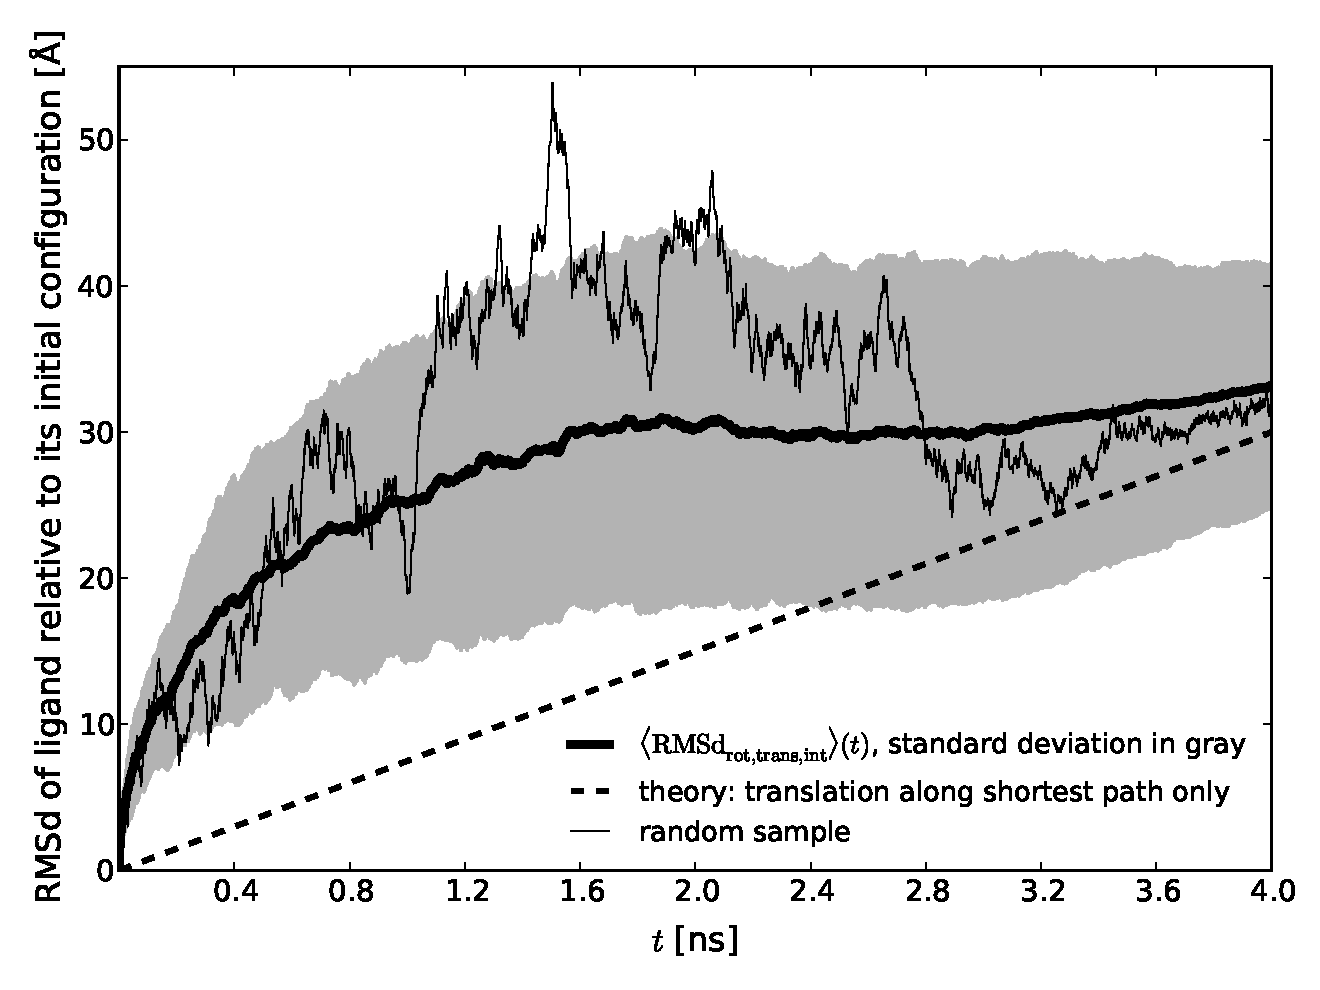
\includegraphics[width=0.9\textwidth]{gfx/dmd/figure_2_freedom_over_time_100samples_avg_stddev_randomone_pub_003.pdf}
\caption[]{
Translational and rotational freedom of a heparin tetramer
while approaching FGF2 during the tMD pulling process with $s=30\,\angstrom$ and
$T=4\,\mathrm{ns}$. For each point in time during tMD, the structural difference between the
current and initial ligand configuration was calculated via classical $RMSd$ and
averaged over 100 independent pulling processes. The variation in ligand
movement among different ligand trajectories is visualized in terms of the standard
deviation (grey background).
}
\label{fig:dmd:sampling}
\end{figure}



For the FGF2-HP complex, we compared tMD runs with different pulling velocities
with the goal to find a moderate velocity which still allows significant
translational and rotational ligand movement. In such a case, entirely different
trajectories among tMD repetitions are produced so that Cartesian space sampling
as well as ligand orientation sampling can be enhanced by increasing the number
of tMD repetitions and leaving all other parameters constant. In tMD test runs
with varying duration $T$ but constant ligand displacement length $s$, we
measured the structural difference ($RMSd$) between the current and initial
ligand configuration for each point in time during tMD. Ligand translation,
rotation and internal conformational changes contribute to this time-dependent
structural difference denoted as $RMSd_{\mathrm{rot,trans,int}}(t)$.  The
difference $RMSd_{\mathrm{rot,trans,int}}(t) - ts/T$ describes the extent of
ligand translation and rotation in space compared to the shortest-path scenario.

For single test cases with $T=4\,\mathrm{ns}$ we observed a quickly fluctuating
$RMSd_{\mathrm{rot,trans,int}}(t)$ curve with ligand displacements from the
shortest path between 5 and $40\,\angstrom$ $RMSd$. In contrast, when using
$T=0.5\,\mathrm{ns}$, the displacement varied in the range between 0 and
$10\,\angstrom$ $RMSd$. From these data, we could already conclude that when
using $T=4\,\mathrm{ns}$, the limiting factor for translational and rotational
ligand sampling is the number of tMD repetitions rather than the pulling
velocity. To further quantify the translational and rotational freedom of the
ligand during tMD with $s=30\,\angstrom$ and $T=4\,\mathrm{ns}$ in detail, we
analyzed the deviation of the ligand from the shortest path for an ensemble of
100 independent tMD runs. To this end, the structural difference between current
and initial ligand configuration was calculated as described above and then
averaged over all 100 independent pulling processes for each point in time
during tMD, leading to $\langle RMSd_{\mathrm{rot,trans,int}}\rangle(t)$
(\cref{fig:dmd:sampling}). The average extent of ligand translation and rotation
in space turned out to have its maximum at an $RMSd$ value of about
$20\,\angstrom$. The path variation among ligand trajectories (the standard
deviation of the averaged data) is about $\pm10\,\angstrom$ $RMSd$. The data
suggest that with $s=30\,\angstrom$ and $T=4\,\mathrm{ns}$ enough translational
and rotational freedom are provided to the ligand during tMD in order to be
applicable in a local docking method. This also verifies that the extend of
sampling of all ligand DOFs is determined and can be adjusted by the number of
tMD repetitions $N$.

$\langle RMSd_{\mathrm{rot,trans,int}}\rangle$ increases slower after about
$t=2\,\mathrm{ns}$ (\cref{fig:dmd:sampling}), which is probably caused by the
electrostatic potential of the receptor prevailing against thermally driven
ligand movement. Having this transition included in the $\langle
RMSd_{\mathrm{rot,trans,int}}\rangle(t)$ curve is a good indication for a
properly (long enough) selected initial displacement length $s$. As a general
rule, $s$ should be chosen in a way that no atoms from the initially placed
ligand lie within the non-bonded interaction cut-off range of the receptor.

Due to the type of distance restraint applied, all final tMD states have the
central ligand atom positioned on the surface of the sphere given by the protein
core atom and the final restraint distance $D$. A more robust realization of the
basic DMD concept would not require assigning specific roles to certain points
(core atom and focus point) but implement a dynamic distance restraint between
receptor surface and ligand during the pulling process.

In the current setup, we have compensated for the spherical – and therefore
limited – distribution of tMD final ligand states via careful selection of the
core atom, of $D$, and via a long free MD simulation stage with
$T=10\,\mathrm{ns}$. This allows for significant ligand refinement according to
the characteristics of the receptor surface as well as for an exhaustive
sampling of the internal DOFs of the ligand. We have quantified the extent of
glycosidic linkage sampling by analyzing the distribution of glycosidic linkage
dihedral values within all free MD simulations of a DMD study with FGF2 in
complex with heparin. Since GLYCAM 06 is known for its proper description of the
glycosidic linkage torsional potential{\cite{kirschner_glycam06:_2008}}, we
extracted the distribution of equivalent torsion angles from an independently
performed 760 ns MD simulation of the same heparin molecule free in solution for
reference. We compared both distributions and observed high similarity between
them (\cref{fig:dmd:glycolinkage_sampling}). In particular, the distribution as
observed for the GAG-only simulation is entirely included in the distribution as
observed from the DMD MD simulations where the GAG is in contact with its
protein receptor. In the latter case, some additional conformers seem to be
accessible to the ligand when compared to the GAG-only simulation, which is to
be expected due to its interaction with the receptor. For further
characterization of the sampling, we extracted glycosidic linkage angle values
from 12 PDB entries containing free heparin as well as heparin-protein complexes
(1AXM, 1BFB, 1BFC, 1E0O, 1FQ9, 1G5N, 1GMN, 1HPN, 1QQP, 2AXM, 2HYU, 2HYV) and
observed that this range of experimentally determined angles is included within
the glycosidic torsion angle distribution as sampled by our MD simulations (also
shown in \cref{fig:dmd:glycolinkage_sampling}).


\begin{figure}
\centering
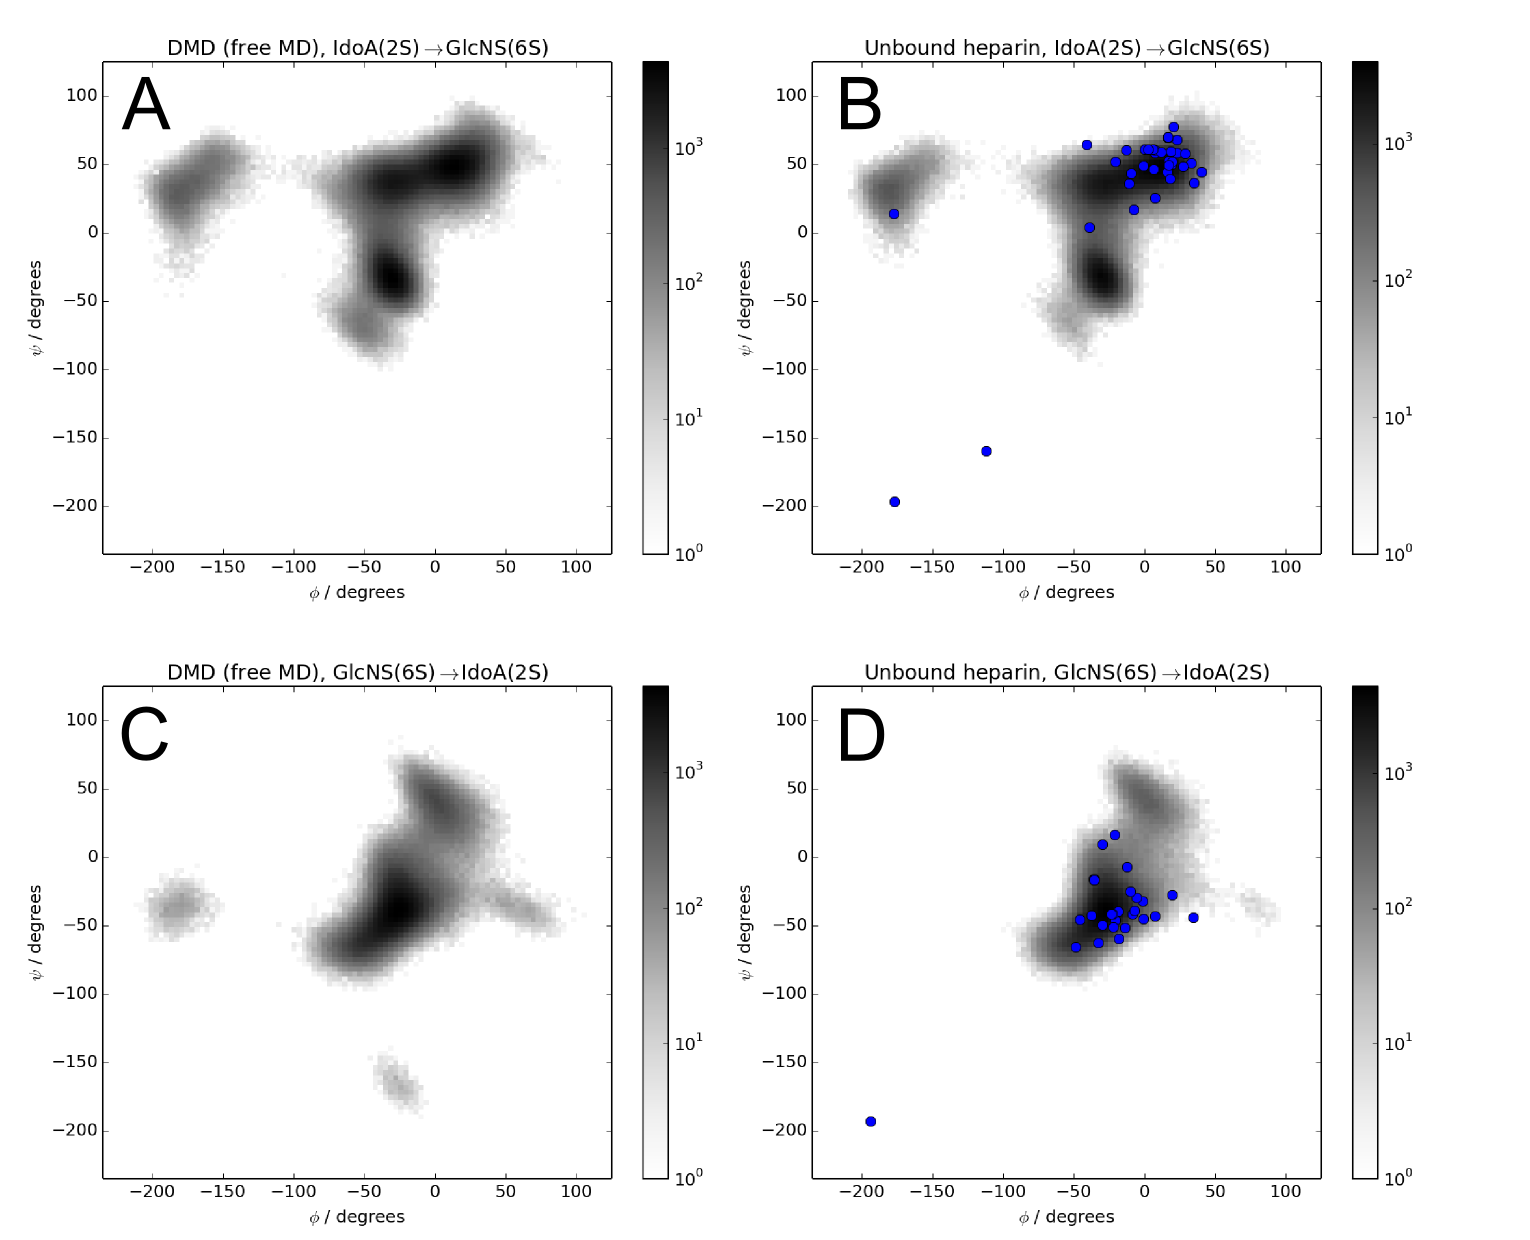
\includegraphics[width=0.9\textwidth]{gfx/dmd/suppl/suppl_glyco_linkage_torsion_maps_03.png}
\caption[]{
Conformational sampling of the glycosidic linkage dihedrals of a free (unbound)
heparin hexasaccharide extracted from 760 ns MD (B, D) compared to the sampling
in all free MD simulations in the DMD study of FGF2-HP (A, C). The torsion
angles are defined as follows: Φ is composed of the atomic chain H1-C1-O4-C4, Ψ
is composed of C1-O4-C4-H4, both in direction from the non-reducing end to the
reducing end of the GAG. All frequency distributions are shown in logarithmic
grey scale. The blue data points in panels B and D additionally show the
distribution of glycosidic linkage dihedral values of heparin as extracted from
the PDB entries 1AXM, 1BFB, 1BFC, 1E0O, 1FQ9, 1G5N, 1GMN, 1HPN, 1QQP, 2AXM,
2HYU, 2HYV (containing unbound as well as bound heparin molecules of different
lengths, the three outliers correspond to terminal sugar monomers).
}
\label{fig:dmd:glycolinkage_sampling}
\end{figure}


Most important, we have observed that due to the long free MD stage and a large
number of DMD repetitions, the overall result of a DMD study becomes insensitive
to moderate changes in focus point coordinates as well as in the final tMD
restraint distance $D$.

When visualizing trajectories of tMD and free MD, we repeatedly observed
conceptually different scenarios. In one type of scenario, the ligand ended up
in its native binding pose in the final state of tMD. The conformation of the
ligand then did not undergo significant changes during free MD. In other cases,
the ligand arrived near its anchoring residues on the surface of the receptor
during tMD and then adopted the native binding mode within the free MD
simulation. We also observed the ligand to end up in a false-positive bound
state as well as in an unbound state after tMD or to unbind during free MD.

From these observations we can deduce that if after DMD no agglomeration of
docking solutions stands out, the chosen receptor target region most likely does
not contain a real binding site for the ligand. Furthermore, even if the focus
point of the method is not centered on but only in the vicinity of a real
binding site, the latter most likely stands out during data analysis.


\subsubsection{Binding site prediction via electrostatic potential analysis}

\hl{Refer back to generic estatic binding site prediction section, explain usage for
DMD. The following paragraphs are duplicates.}

Regarding the SDF-1-HP complex, our electrostatic potential evaluation procedure
unambiguously identifies the GAG binding site as determined experimentally. With
$8.5\,\mathrm{kcal\,mol^{-1}\,e^{-1}}$, the isovalue chosen is the largest among
the TDS complexes, indicating that SDF-1 has the strongest electrostatic
attraction to its ligand. In case of FGF2-HP
(\cref{fig:bspred:various_estatic}), the binding site is also unambiguously
defined by the electrostatic potential. For CD44-HA, the net electrostatic
interaction between both molecules is slightly repulsive. There is no obvious
relation between the electrostatic properties of the receptor and the binding
site location. CathK and CathKmut exhibit electrostatic attraction for
negatively charged molecules in the experimentally observed ligand binding site
as well as in an adjacent region. We observe that electrostatic potential
analysis provides a clear idea whether GAG-binding to a given receptor is mainly
driven by Coulomb interaction. If a protein is known to bind GAGs, and the
electrostatic potential topology is as unambiguous as in case of SDF-1 or FGF2,
a GAG binding site prediction based on the presented procedure is reliable.
Visualization of the electrostatic potential can also be helpful to \textit{a
priori} exclude regions of the receptor surface when repulsive to negatively
charged ligands. Furthermore, this analysis shows that knowledge about the
electrostatic potential distribution in space can be used to choose a reasonable
ligand \enquote{entry lane} orientation for the tMD pulling process.


The SH3-p41 complex is dominated by non-polar interactions, rendering the
Coulomb potential analysis inconclusive. Recognition of the Trypsin inhibitor in
its  binding pocket is affected by polar interactions. The electrostatic
potential, however, does not display clear characteristics to predict a binding
region.

\subsubsection{DMD performance}

{\sffamily Spatial distribution of docking solutions.}

\begin{figure}
\centering
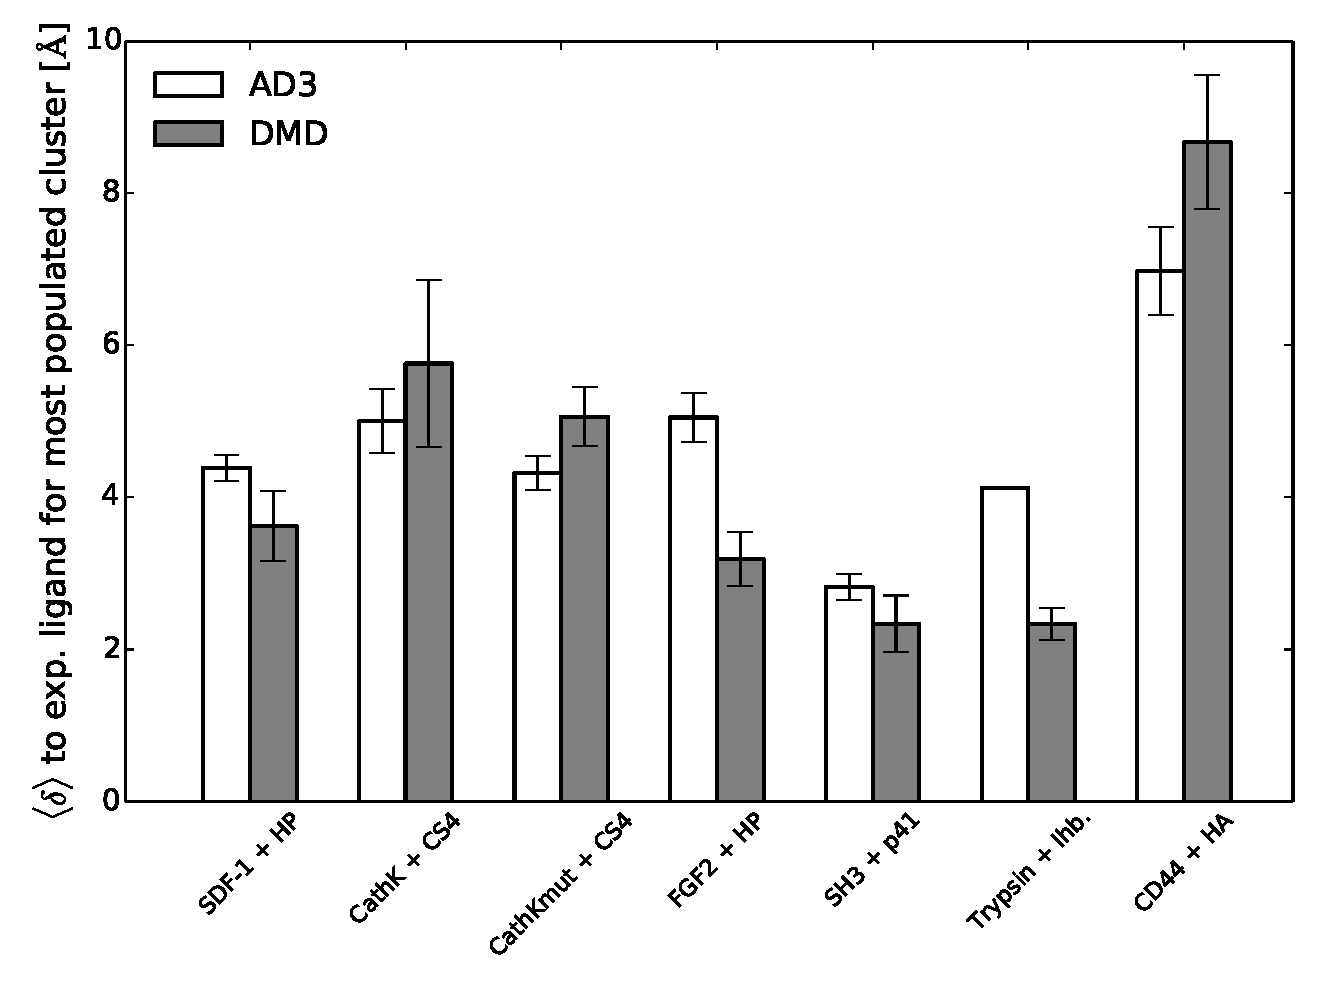
\includegraphics[width=0.9\textwidth]{gfx/dmd/figure_4_clustering_dmd_vs_ad3_plots_pub_004.pdf}
\caption[]{
Mean structural distance $\langle \delta \rangle$ between all members of the
most populated cluster and the experimentally determined ligand for all
investigated complexes with both docking methods. The error bars show the
standard deviation of the mean.
}
\label{fig:dmd:clus_dmd_vs_ad3}
\end{figure}



\begin{table}
\tiny
\centering
\renewcommand{\arraystretch}{1.3}
\begin{tabular}{@{}lcccc@{}}
\multicolumn{5}{c}{\textbf{DMD}} \\
\midrule
Complex & $\epsilon$ / \angstrom & members & $\delta$ / \angstrom (mean) &  $\delta$ / \angstrom (std. dev.) \\
\midrule
CathKmut + CS4 & 3.0 & 6   & 5.1 & 0.4 \\
CathK + CS4    & 3.0 & 4   & 5.8 & 1.1 \\
SDF1 + HE      & 2.2 & 8   & 3.6 & 0.5 \\
CD44 + HA      & 3.2 & 5   & 8.7 & 0.9 \\
SH3 + p41      & 2.6 & 8   & 2.3 & 0.4 \\
FGF + HE       & 2.5 & 6   & 3.2 & 0.4 \\
Trypsin + Ihb. & 1.0 & 9   & 2.3 & 0.2 \\
\midrule
& & & & \\
\multicolumn{5}{c}{\textbf{AD3}} \\
\midrule
Complex & $\epsilon$ / \angstrom & members & $\delta$ / \angstrom (mean) &  $\delta$ / \angstrom (std. dev.) \\
\midrule
CathKmut + CS4  & 2.5 & 6   & 4.3 & 0.2 \\
CathK + CS4     & 2.0 & 9   & 5.0 & 0.4 \\
SDF1 + HE       & 1.2 & 19  & 4.4 & 0.2 \\
CD44 + HA       & 2.5 & 8   & 7.0 & 0.6 \\
SH3 + p41       & 1.8 & 10  & 2.8 & 0.2 \\
FGF + HE        & 1.6 & 10  & 5.1 & 0.3 \\
Trypsin + Ihb.  & 0.1 & 100 & 4.1 & 0.0 \\
\midrule
\end{tabular}
\caption{
Clustering parameters of the most populated cluster for docking solution
ensembles obtained via DMD and AD3. $\epsilon$ is the neighborhood search radius
as used for DBSCAN clustering, $\delta$ measures the structural difference
between two molecules (see Methods).
}
\label{tab:dmd:clustering_parameters}
\end{table}


We compared the performance of DMD with the performance of the well-established
AD3 docking approach, which was used for other molecular systems including GAGs.
We applied DMD and AD3 to all TDS complexes and analyzed the spatial
distribution of docking results via clustering
(\cref{tab:dmd:clustering_parameters} \hl{remove this table?}). For each
complex, we compared the mean structural distance $\langle \delta \rangle$
between the experimentally determined ligand position and all members of the
most populated cluster (\cref{fig:dmd:clus_dmd_vs_ad3}). In terms of the
capability to produce solutions structurally close to the experimentally
determined ones, both docking methods perform comparably well. However,
interesting differences are observable. AD3 generally yields smaller spatial
scattering of solutions as given by the standard deviation of data points in
\cref{fig:dmd:clus_dmd_vs_ad3}. This can be attributed to the static treatment
of the receptor by AD3. Notably, we can generally conclude that DMD performed
better than AD3 for the complexes with strongest electrostatic attraction,
namely SDF-1-HP and FGF2-HP. For the FGF2-HP complex, the most populated cluster
from DMD reproduces the experimentally determined HP binding pose, while the
most populated cluster from AD3 docking only partially overlaps with this pose
(\cref{fig:dmd:fgf2zoom}a). In fact, DMD was able to identify the
\enquote{higher affinity} binding site for heparin (as denoted in the original
publication of the FGF2-HP crystal structure), while AD3 identified the
\enquote{lower affinity} site, which becomes occupied upon heparin
hexasaccharide binding \cite{faham_heparin_1996}. In addition, DMD was able to
properly predict the positioning of the two sulfate groups making specific high-
affinity contact to FGF2 (\cref{fig:dmd:fgf2zoom}b). These two sulfate groups
form seven of the nine polar contacts between FGF2 and HP and therefore are
important anchoring groups for the molecular recognition
\cite{faham_heparin_1996}. The fact that DMD was able to reproduce this key
feature as opposed to AD3 most probably reflects the crucial role of receptor
flexibility considered in the docking simulation.

\begin{figure}
\centering
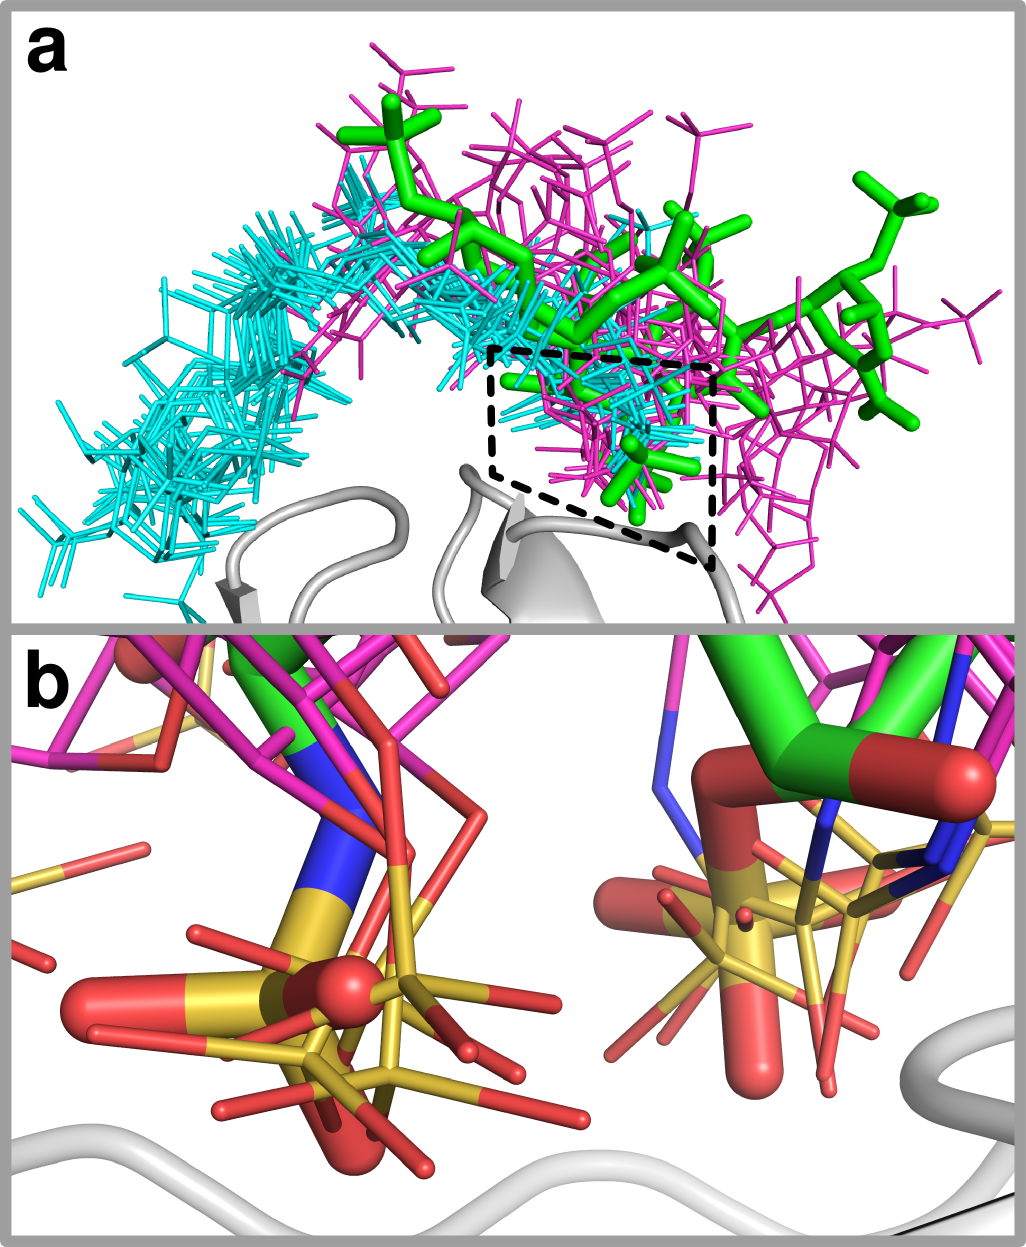
\includegraphics[width=0.9\textwidth]{gfx/dmd/fgf2_topclusters_dmd_vs_ad3_receptorribbon_normal_and_zoom_jcc_004.png}
\caption[]{
Docking results from DMD and AD3 for FGF2 (grey cartoon representation) and HP.
\textbf{a}: ligand from crystal structure in green sticks. Most populated
cluster of DMD solutions in magenta. Most populated cluster of AD3 solutions in
cyan. \textbf{b}: zoom on two sulfate groups making specific high-affinity
contact to FGF2 \cite{faham_heparin_1996} (as marked in \textbf{a} via dashed
line). Ligand from crystal structure with C atoms in green (thick sticks). Most
populated DMD cluster with C atoms in magenta (thin sticks).
}
\label{fig:dmd:fgf2zoom}
\end{figure}


In order to assess the ability of DMD to predict consistent binding poses for
GAGs differing in length, we carried out additional DMD studies for SDF-1 as
well as FGF2. Eventually, both systems were investigated with independent DMD
studies for each of di-, tetra- and hexasaccharides of heparin. For FGF2-HP, the
two sulfate groups making specific contact to FGF2 were identified when docking
both an HP tetrasaccharide and an HP hexasaccharide. These observations support
the assumption that GAG fragments differing in length share key interactions
with the protein. When docking an HP disaccharide, those key interactions were
not identified, suggesting that the disaccharide is not long enough to maintain
specificity. Nevertheless, for the SDF-1-HP and FGF2-HP systems, we observe that
all obtained poses overlap regardless of GAG length (\cref{fig:dmd:fgf2_hp_246,%
fig:dmd:sdf1_hp_246}).  A direct visual comparison between the crystal structure
of FGF2 with a heparin hexasaccharide{\cite{faham_heparin_1996}} and the
corresponding DMD result can be seen in \cref{fig:dmd:fgf2_hp_246}.


\begin{figure}
\centering
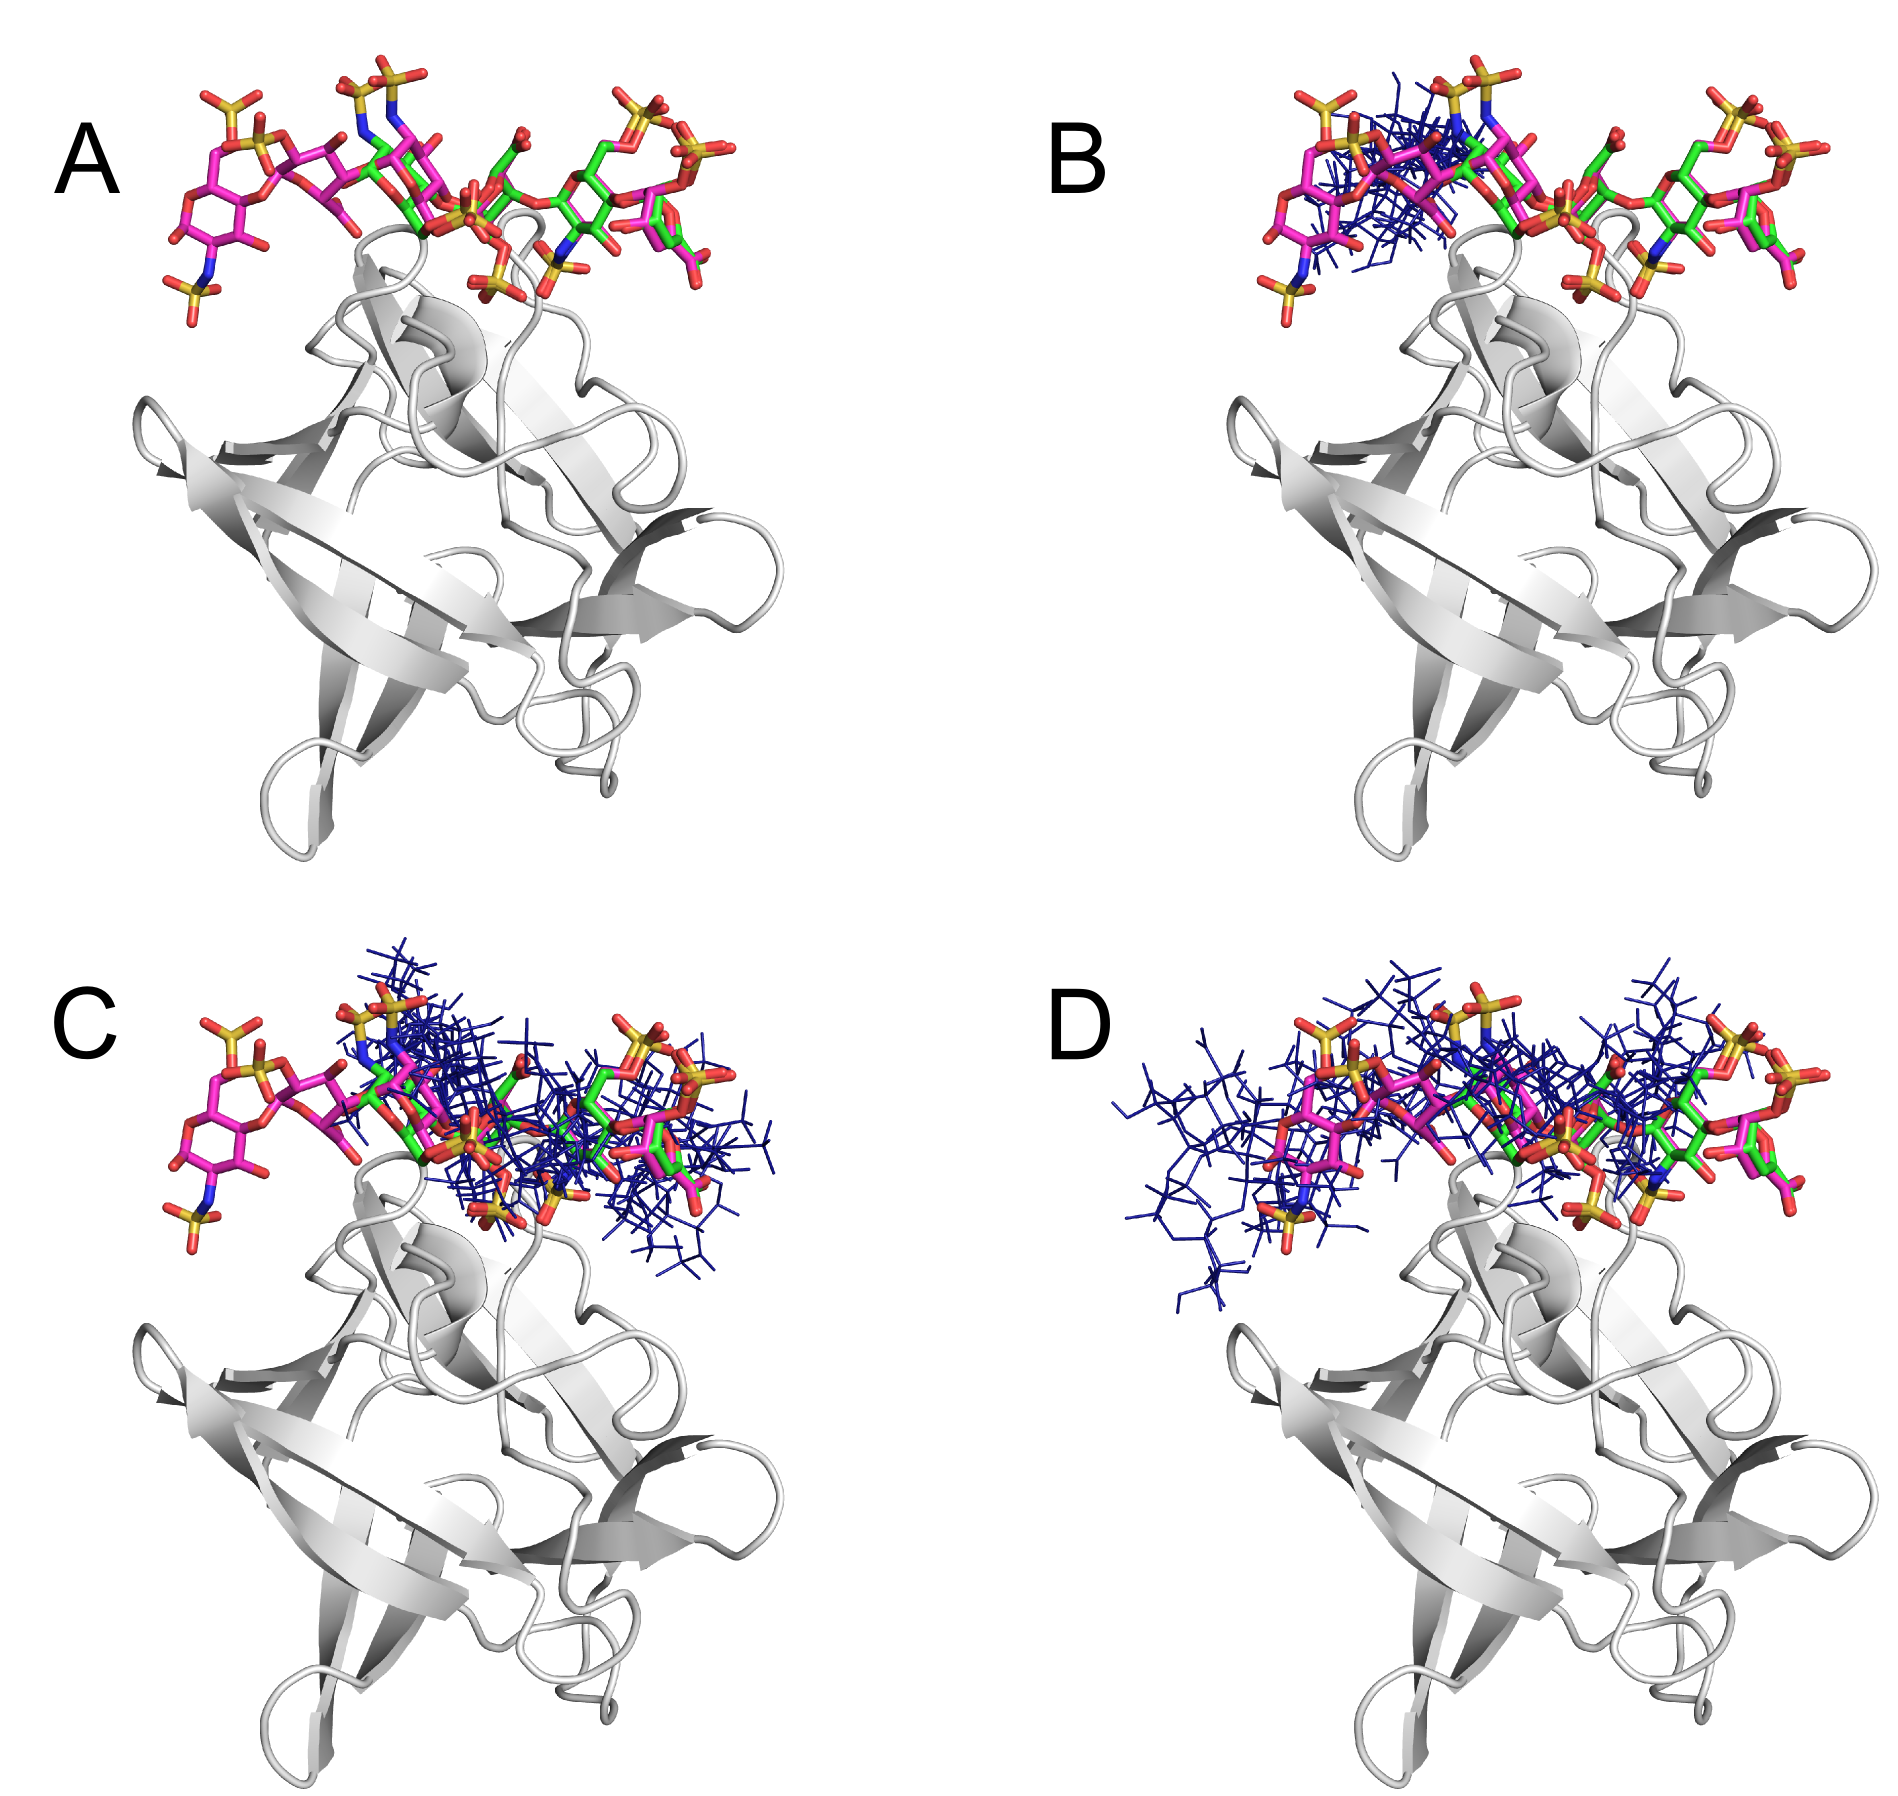
\includegraphics[width=0.9\textwidth]{gfx/dmd/suppl/suppl_fgf2_dmd_he-2-4-6_02.png}
\caption[]{
DMD results for FGF2 in complex with a heparin di-, tetra- and hexasaccharide.
In magenta and green sticks, the heparin hexamer and tetramer poses as
determined experimentally are shown (PDB IDs 1BFB, 1BFC), respectively. The most
populated clusters for di-, tetra- and hexasaccharide docking solutions are
shown in B, C, D, respectively, as blue sticks. The protein is shown in grey
cartoon.
}
\label{fig:dmd:fgf2_hp_246}
\end{figure}


\begin{figure}
\centering
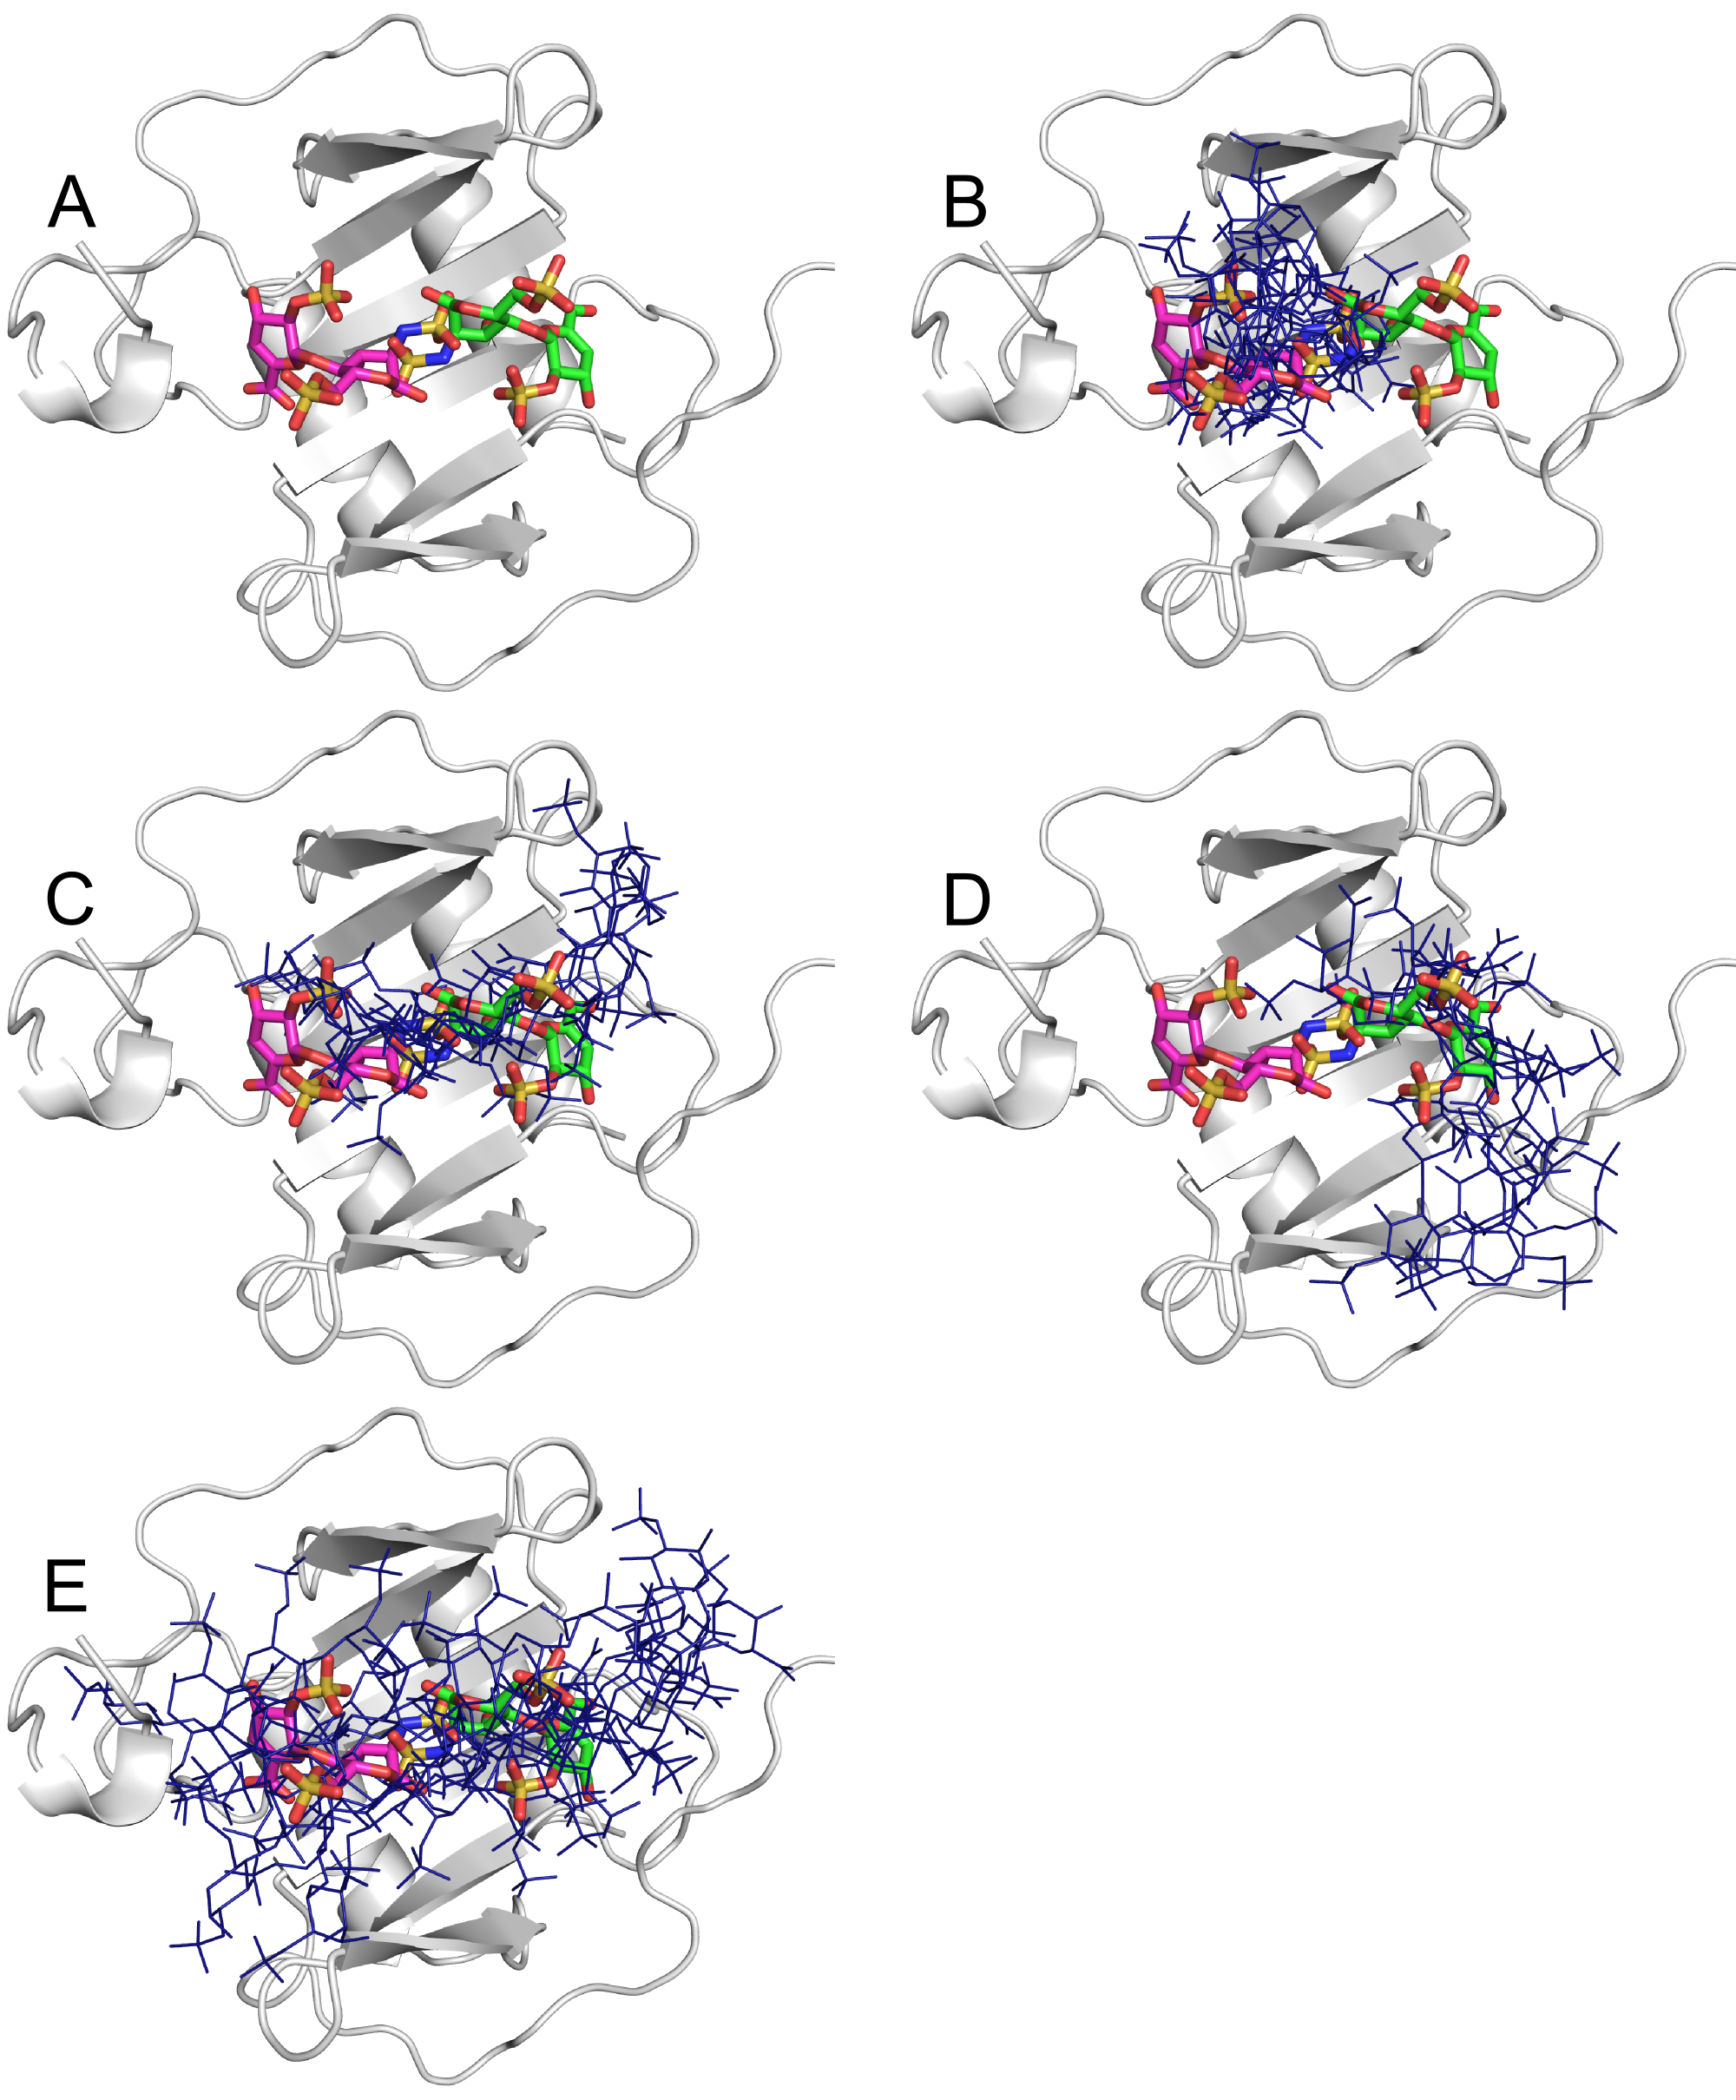
\includegraphics[width=0.9\textwidth]{gfx/dmd/suppl/suppl_sdf1_dmd_he-2-4-6.png}
\caption[]{
DMD results for SDF-1 in complex with a heparin di-, tetra- and hexasaccharide.
In magenta sticks, the heparin dimer pose as determined experimentally is shown
(PDB ID 2NWG). For clarity, we show its symmetric counterpart (180 degree
rotation about the 2-fold axis of the SDF-1 dimer) in green sticks. The most
populated clusters for di-, tetra- and hexasaccharide docking solutions are
shown in B, C \& D, E, respectively, as blue sticks. The protein is shown in
grey cartoon.
}
\label{fig:dmd:sdf1_hp_246}
\end{figure}


As has been conceptually described for the FGF2-HP complex, also regarding the
SH3-p41 and Trypsin-inhibitor complexes, DMD provided solutions closer to the
experimentally determined ones while displaying a more diverse scattering of
docking solutions than AD3.

For CD44 in complex with the HA heptamer, both docking methods were only
partially able to reproduce the experimentally determined ligand pose. Weak net
electrostatic repulsion between receptor and ligand seemingly imposes a major
challenge for both docking methods. AD3 and DMD solutions, however, are
spatially consistent (data not shown).

Both docking methods had difficulties reproducing the experimentally determined
binding poses of CathK and CathKmut in complex with CS4. In case of CathK-CS4,
the crystal structure contains a single high molecular weight polymeric CS4
molecule interacting with multiple copies of the same protein
\cite{catK_cs4_crystal_structure_2008}. Within the CathKmut-CS4 crystal, each
GAG hexamer tightly interacts with two CathKmut proteins
\cite{catKmut_cs4_crystal_2011}. Under these conditions, it is to be expected
that considering only a short GAG and a single protein in the docking experiment
is not sufficient to allow for an accurate reproduction of the experimentally
determined structures.

The presented structural difference comparison between DMD and AD3-based docking
solutions and the corresponding experimentally determined ligand coordinates is
subject to a systematic error. Structural relaxation prior to docking with AD3
changed the receptor side chains in the binding region by a heavy atom $RMSd$ of
$(1.0\pm0.4)\,\angstrom$ (mean value and standard deviation derived from all TDS
complexes) when compared to the experimentally determined receptor structure.
The solutions from DMD display a mean binding region alteration of
$(2.3\pm0.6)\,\angstrom$ (corresponding raw data is shown in
\cref{tab:dmd:binding_site_rmsd}). The larger the binding site
alteration, the more error-prone the comparison between docked solution and
experimentally determined ligand becomes. Under the assumption that this error
systematically increases the structural difference, DMD might have performed
better compared to AD3 than shown in Figure 4.


% http://www.inf.ethz.ch/personal/markusp/teaching/guides/guide-tables.pdf
\begin{table}
\tiny
\centering
\renewcommand{\arraystretch}{1.3}
\begin{tabular}{@{}lcccc@{}}
\toprule
& \multicolumn{2}{c}{\textbf{DMD (after free MD)}} & \multicolumn{2}{c}{\textbf{AD3}} \\
Complex & Entire receptor & Binding site &  Entire receptor & Binding site \\
\midrule
SDF-1 + HP & 3.6 $\pm$ 0.5 & 2.3 $\pm$ 0.5 &  0.4 & 0.2 \\
CathK + CS4 & 1.8 $\pm$ 0.2 & 2.0 $\pm$ 0.3 & 1.1 & 1.2 \\
CathKmut + CS4 & 1.8 $\pm$ 0.2 & 1.9 $\pm$ 0.4 & 1.1 & 1.4 \\
FGF2 + HP & 3.4 $\pm$ 0.1 & 3.6 $\pm$ 0.1 & 1.3 & 1.1 \\
SH3 + p41 & 2.2 $\pm$ 0.2&  2.4 $\pm$ 0.4 &  1.3 & 1.4 \\
Trypsin + Ihb. & 1.6 $\pm$ 0.1 & 1.5 $\pm$ 0.4 & 0.9 & 0.7 \\
CD44 + HA & 2.2 $\pm$ 0.3 & 2.5 $\pm$ 0.5 & 0.9 & 0.7 \\
\bottomrule
\end{tabular}
\caption{
Heavy atom RMSd between experimentally determined structure of the receptors and
the receptor structures corresponding to the docking solutions. Differences were
obtained for \textit{i} the entire receptor and \textit{ii)} the binding site
only as determined by the MOE \enquote{pocket} feature. In case of DMD, mean
distances $\pm$ standard deviation were obtained from 100 independent free MD
runs per complex. Numbers are given in ångströms.
}
\label{tab:dmd:binding_site_rmsd}
\end{table}


{\sffamily Energetic evaluation of docking results}

% TODO
Lose a word or two on the meaningfulness of MMPBSA score for single
solutions.

% {\sffamily \small Scoring.} It is well-established to assign an energy-related
% score to each obtained docking solution allowing for an energetic ranking of
% such. While AD3 provides its own scoring scheme, we built two different score
% values per DMD docking solution: the Coulomb energy $\Delta E$ between receptor
% and ligand as well as an MM-PBSA estimate for the free energy of binding,
% $\Delta G$ (as described in Methods).

% Although debatable, in order to validate a scoring method, the rank by score is
% often expected to decrease with increasing distance between the ideal solution
% and the scored docking solutions \cite{plewczynski_can_2011}. We calculated
% Spearman's rank correlation between $\delta$ and AD3 score, DMD $\Delta G$, DMD
% $\Delta E$ for all TDS complexes. For each scoring method, two Spearman
% coefficients were determined based on two different docking solution subsets:
% the first subset included all solutions with $\delta \le 20\,\angstrom$, the
% solutions in the second subset fulfill  $\delta \le 6\,\angstrom$. Coefficients
% have been calculated only when at least eight value pairs were available.
% Between the two distance filter cases, the resulting correlation coefficients
% varied significantly: For both DMD scoring methods, we generally observed higher
% coefficients for $\delta \le 20\,\angstrom$ than for $\delta \le 6\,\angstrom$
% in case of the four protein-GAG complexes dominated by electrostatic attraction
% (FGF2-HP, SDF-1-HP, CathK-CS4, CathKmut-CS4, see Supplementary Figure 2). This
% is an effect of long-range electrostatic potential, which slowly decays with
% increasing distance from the GAG binding site. Within the vicinity of the
% experimentally determined ligand position ($\delta \le 6\,\angstrom$), we
% observed that only DMD $\Delta E$ yielded a correlation coefficient larger than
% 0.2 for most of the complexes. From the data we can not derive a clear relation
% between $\delta$ and any of the scoring metrics.

% In order to analyze the influence of GAG length on the DMD $\Delta G$ score, we
% investigated the MM-PBSA results of our DMD studies with SDF-1 and FGF2 in
% complex with heparin di-, tetra- and hexasaccharides. We observe that the free
% energy of binding estimates becomes more favorable with increasing GAG length:
% the average $\Delta G$ values in kcal/mol for the most populated clusters of
% SDF-1-HP are -59.2, -96.7, -144.4 and of FGF2-HP are -37.0, -73.8, -80.4 for
% di-, tetra- and hexasaccharides, respectively. For FGF2, the difference between
% the values for hexa- and tetrasaccharide is rather small compared to the
% difference between values for tetra- and disaccharide. This is in agreement with
% experimental data showing that a heparin tetrasaccharide is sufficient to occupy
% the high affinity part of the FGF2 heparin binding
% site{\cite{faham_heparin_1996}}.

%TODO: Properly implement hierarchy level.
\textbf{Identification of anchoring residues in the ligand binding
region.} The prediction of receptor residues important for ligand binding is of
particular practical value. While AD3 does not provide energetic data on the
single-residue level, DMD allows for a single-residue energy decomposition
(SRED) based on time-averaged free MD interaction energy data.


For each TDS complex, we merged SRED data from the entire ensemble of DMD runs
and extracted the set of anchoring residues, which are at most ten of the
receptor residues contributing most (positively) to ligand binding. We also
determined a reference set of anchoring residues from MD simulations of the
experimentally determined structures. For each TDS complex, we then identified
the intersection of both sets (Table 1).


For Trypsin in complex with its inhibitor, half of the anchoring residues in the
crystal structure were correctly found. For SDF-1-HP, CathK-CS4, and CathKmut-
CS4 more than half of the anchoring residues were identified by SRED.
Furthermore, for the FGF2-HP complex, nine of ten anchoring residues were
predicted properly.

In order to evaluate the capability of DMD to rank the receptor anchoring
residues according to their importance for ligand binding, we calculated
Spearman's rank correlation between the SRED-energies of residues in both, the
reference and comparison sets (Table 1). For three of those five complexes with
at least five predicted anchoring residues, the DMD ranking turned out to
reproduce the reference ranking quite well (SDF-1-HP, FGF2-HP, Trypsin-Ihb). For
the CathK-CS4 and CathKmut-CS4 complexes the anchoring residue ranking was not
reproduced.

\begin{figure}
\centering
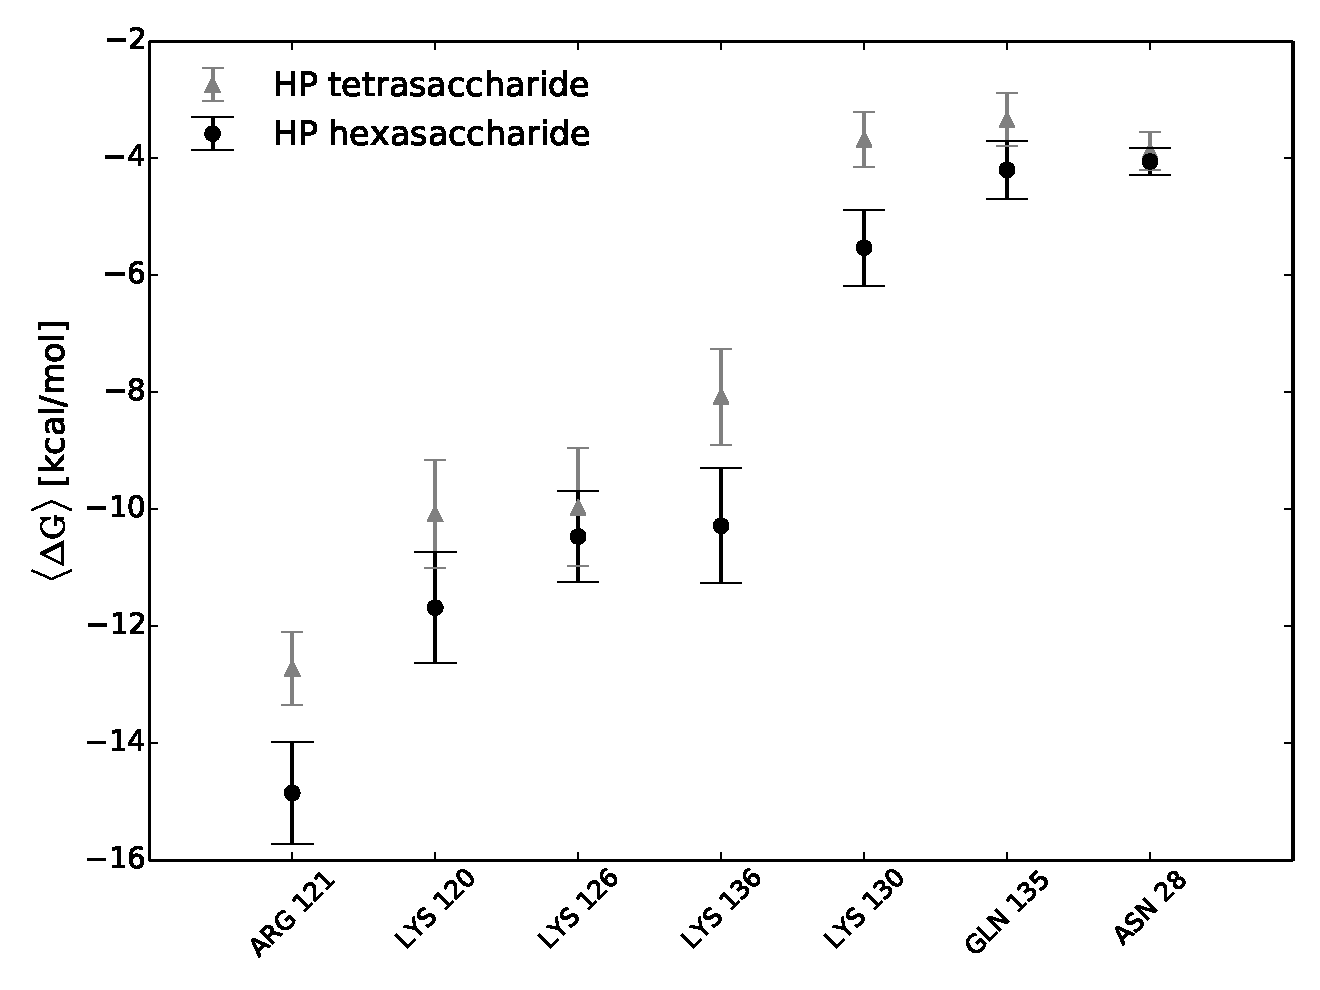
\includegraphics[width=0.9\textwidth]{gfx/dmd/figure_6_receptor_top7_residues_of_top_40percent_dmd_runs.pdf}
\caption[]{
FGF2 amino acid residues identified by DMD as having the greatest impact on
FGF2-HP binding. Results are shown for both heparin tetra- and hexasaccharide
ligands as retrieved from two independent DMD studies. For each residue, an
average energy ($\pm$ standard error of the mean) for the interaction with the
ligand is shown as obtained from 40 independent free MD simulations.
}
\label{fig:dmd:sred_fgf2}
\end{figure}

Based on the obtained results, we can conclude that for systems dominated by
electrostatic attraction such as protein-GAG systems, DMD is capable of
correctly identifying those amino acid residues responsible for forming key
interactions with the ligand. Regarding the FGF2-HP system, we found that both
heparin tetra- and hexasaccharide docking via DMD enabled us to consistently
identify the same chemical groups in the GAG molecule being key for binding.
Moreover, using SRED data, we were able to demonstrate that the identified key
amino acid residues as well as their energy ranking are identical when comparing
heparin tetra- and hexasaccharide docking performed in independent DMD studies
(see \cref{fig:dmd:sred_fgf2}). This observation supports the idea that,
regardless of their length, GAG fragments preserve their key interactions with
certain protein amino acid residues. The set of FGF2 key amino acid residues as
identified by SRED contains all residues that were crystallographically
characterized as most important for binding (R121, K126, N28,
Q135){\cite{faham_heparin_1996}}. Based on our data we can additionally state
that also residue K120 is of major importance, since it acts as hydrogen bond
donor in a similar way as K126 does. The latter observation is in agreement with
previous calorimetry studies pointing out the importance of K120 in the FGF2-HP
system{\cite{thompson_1994_fgf2_heparin}}. These findings motivate the
application of DMD to systems in which a detailed and appropriate description of
GAG recognition is required.

% TODO: clarify hierarchy? remove parts?
\vspace{1.5cm} In summary, our data suggest that DMD is able to yield docking
results of high significance, especially in case of receptor-ligand systems
dominated by attractive electrostatic interaction. This success is well-grounded
by the concept of the ligand conformational sampling while responding to the
long-range Coulomb potential of the receptor when slowly approaching its
surface. During this step, the Coulomb potential significantly contributes to
steering the entirely flexible and charged ligand towards its binding site and
to let it finally adopt its binding pose in an explicit solvent environment. The
subsequent free MD step allows for an unbiased mutual adjustment of receptor
residues and ligand.

DMD is a local docking method focused towards a certain region on the receptor
surface. If the confidence in the binding region assumption is to be increased,
one could repeat the DMD study while varying the focus point for covering a
larger search space. There is no general dependence of the DMD protocol on the
confidence in the binding region assumption (however, the conclusiveness of the
DMD results clearly depends on the validity of this assumption). When selecting
focus point, core atom, and target distance $D$, one needs to ensure that after
the pulling process, the ligand is able to establish short-range interactions
within the receptor binding region but is not forced into clashes with the
receptor. In our study, we selected the focus point based on the experimentally
determined ligand position (\cref{tab:dmd:tds_target_distances}). \hl{In practice,
when the structure of the bound ligand is unknown, the focus point has to be
defined based on the residues comprising the putative binding region. Via
analysis of the atomic coordinates of ten protein-GAG complexes (PDB IDs 1BFB,
1G5N, 1GMO, 1RID, 1T8U, 2BRS, 2HYU, 2JQR, 3C9E, 1XMN, including GAGs comprised
of two to seven monosaccharide units), we found that the distance as well as the
direction from the center of mass of the receptor residues comprising the
putative binding site to the ligand center is consistent within these complexes
(Supplementary Table 2). This relationship can be used to derive a focus point
from the residues constituting the receptor binding region.\textbf{REMOVE?}}

\begin{table}
\scriptsize
\centering
\renewcommand{\arraystretch}{1.3}
\begin{tabular}{@{}lr@{}}
\toprule
Complex & $D$ / \angstrom \\
\midrule
SDF-1 + HP & 10.6 \\
CathK + CS4 & 19.2 \\
CathKmut + CS4 & 20.9 \\
FGF2 + HP & 25.0 \\
SH3 + p41 & 7.7 \\
Trypsin + Ihb. & 12.1 \\
CD44 + HA & 15.3 \\
\bottomrule
\end{tabular}
\caption{
Target distance $D$ as applied during the tMD simulations for any given TDS complex.
}
\label{tab:dmd:tds_target_distances}
\end{table}


One of the main concepts of DMD is that pulling process and subsequent free MD
are repeated many times in independent simulations. This allows for the creation
and evaluation of an ensemble of docking solutions rather than the
interpretation of single trajectories. In this ensemble, the energetically more
favorable states are the more likely ones. Spatial clustering of this docking
solution ensemble identifies those docking solutions that appeared with highest
probability and, therefore, lowest energy. With respect to the identification of
anchoring residues in the receptor and their energetical ranking, meaningful
results can be obtained by merging the properties of multiple docking solutions.

Sampling performance is one of the main limitations of any docking method.
Regarding our DMD protocol applied to the TDS complexes, we have shown that with
100 independent DMD runs the sampling performance was sufficient for generating
meaningful docking solution ensembles. Although the predictive significance of
DMD in this study has been good enough, it can still be largely improved by a
sampling enhancement. An obvious way for achieving this would be to increase the
number of independent DMD runs, which would result in an even clearer picture
upon clustering of a docking solution ensemble. Furthermore, the current DMD
protocol leaves room for optimizing the sampling performance per compute time
via careful reduction of the ligand starting distance and increase of the
pulling velocity.

Beyond the proof of concept provided by this study for including receptor
flexibility and explicit solvent in molecular dynamics-based docking of protein-
GAG systems, the analysis of MD data collected in the course of DMD can be
largely extended to further increase the atomic resolution of results, improve
the overall predictive significance and to gain new insights into molecular
recognition mechanisms. The behavior and role of single water molecules in
ligand binding, for instance, could be investigated thoroughly. Furthermore, the
dynamic nature of DMD data enables and motivates the creation of specialized
scoring schemes, e.g.\ the evaluation of ligand position fluctuations during
free MD as an indicator for the stability of a docking solution. Also, the
single-residue energy decomposition analysis can be accompanied by an evaluation
of hydrogen bond formation and occupancy via simple distance and angle criteria.

An important challenge in GAG-protein docking is to properly deal with the
conformational flexibility of IdoA(2S) in
heparin\cite{Mulloy_dyn_conf_heparin_2000, barbero_jacs_2005}. Unfortunately,
GLYCAM 06 is known to not properly reproduce the natural ring conformer
population of IdoA(2S) \cite{gandhi_idoa2s_2010} and its ring conformation
interconversion time scale is beyond simulation times accessible in DMD
anyway{\cite{almond_jacs_2010}}. Nevertheless, this issue can be addressed by
applying ring-internal restraints to explicitly impose a certain conformation on
individual rings (as outlined in the Methods section) and then perform a number
of independent DMD studies differing only in the combination of ring
conformations -- an approach which has recently been proposed by Mu\~noz-
Garc\'ia and co-workers{\cite{conf_idoa_timeavg_restraints_2013}}. As we have
shown previously, the MM-PBSA approach is capable of distinguishing GAG poses
differing only in the conformation of one single
ring \cite{Samsonov_rings_cr_2013}.

Although the computational demands for DMD are higher than for conventional
docking methods such as AD3, investigations of single systems via DMD are
entirely feasible when having access to reasonable computing resources,
especially using MD software optimized for GPU hardware such as Amber: a DMD
study for the FGF2-HP complex as presented here can be performed within one week
incorporating six modern GPU cards (GTX 580 in this case).

%((Equations should be inserted using standard LaTeX equation and eqnarray environments, not as graphics, and should be set in the main text))
%Equation                                           (1)
%((References should be superscripted and appear after punctuation.1,2 Please define all acronyms at their first usage except IR, UV, NMR, and DNA or similar commonly understood terms.))


%\subsection*{\sffamily \large Second-order heading}
%\subsubsection*{\sffamily \normalsize Third-order heading}
%{\sffamily \small Fourth-order heading}\\

\subsection{Conclusions}

In this study, we have established and tested DMD, a targeted molecular
dynamics-based protocol for local docking developed for specifically tackling
the challenges imposed by highly flexible systems dominated by electrostatic
interaction, such as protein-GAG systems.

In particular, flexible treatment of the receptor copes with the fact that GAGs
usually bind to charged surface patches on the receptor comprised of highly
flexible side chains. The identification of proper binding poses in these
surface patches requires the flexible adjustments of protein residues to the GAG
ligand. Furthermore, the inclusion of explicit solvent in DMD considers the
solvent-accessibility of such binding sites and -- most important -- lives up to
the supremacy of charge-charge interactions in most protein-GAG complexes. The
dominating long-range Coulomb potential is explicitly exploited as a driving
force in DMD while slowly approaching the ligand towards the receptor. A long
free MD step and the flexible treatment of the ligand allow for an extensive
sampling of the GAG-internal degrees of freedom.

We show that DMD has high predictive significance for systems dominated by
electrostatic attraction. Our data implicate that via proper selection of DMD
parameters such as pulling velocity, ligand displacement distance and the number
of independent repetitions, sufficient sampling is achievable. We demonstrate
that in some cases the simple analysis of the spatial distribution of the
electrostatic potential of the receptor can lead to a reliable prediction of the
GAG binding region and therefore offers itself as a useful tool for defining the
target region on the receptor surface as required by DMD.

Regarding the spatial distribution of docking solutions, DMD generally yields
results comparable to AD3. Nevertheless, DMD performs better in terms of
achieving agreement with atomic details inferred from experimental data. The
time-dependent data obtained via DMD allows for a reliable prediction of
receptor anchoring residues via MM-PB(GB)SA single-residue energy decomposition,
yielding consistent results when docking GAGs of different length. Furthermore,
obtained MD trajectory data pave the way for the evaluation of various dynamics-
based measures, the development of specialized scoring schemes, and the
investigation of the dynamic nature of molecular interaction mechanisms within a
particular system.
